%%%%%%%%%%%%%%%%%%%%%%%%%%%%%%%%%%%%%%%%%%%%%%%%%%%%%%%%%%%%%%%%%%%%%%%%%%%%%%%%%%%%%%%%%%%%%%%%%%%%%%%%%%%%%%%%%%%%%%%%%%%%%%%%%%%%%%%%%%%%%%%%%%%%%%%%%%%%%%%%%%%%%%%
%%%%%%%%%%%%%%%%%%%%%%%%%%%%%%%%%%%%%%%%%%%%%%%%%%%%%%%%%%%%%%%%%%%%%%%%%%%%%%%%%%%%%%%%%%%%%%%%%%%%%%%%%%%%%%%%%%%%%%%%%%%%%%%%%%%%%%%%%%%%%%%%%%%%%%%%%%%%%%%%%%%%%%%
%%%%%%%%%%%%%%%%%%%%%%%%%%%%%%%%%%%%%%%%%%%%%%%%%%%%%%%%%%%%%%%%%%%%%%%%%%%%%%%%%%%%%%%%%%%%%%%%%%%%%%%%%%%%%%%%%%%%%%%%%%%%%%%%%%%%%%%%%%%%%%%%%%%%%%%%%%%%%%%%%%%%%%%
\chapter{Simulated samples}
\label{sec:SimulatedSamples}

In order to design the search and to study background and signal characteristics, this analysis relies on simulated  SM and SUSY datasets.
An extensive introduction to the techniques and tools required for the simulation of SM and beyond SM processes can be found in Section~\ref{FIXME}.

The following two sections present an overview of the SM (Section~\ref{sec:SMSamples}) and SUSY samples (Section~\ref{sec:SignalSamples}) used in this search.
All samples are reweighted to match the measured distribution of primary vertices in data.

%%%%%%%%%%%%%%%%%%%%%%%%%%%%%%%%%%%%%%%%%%%%%%%%%%%%%%%%%%%%%%%%%%%%%%%%%%%%%%%%%%%%%%%%%%%%%%%%%%%%%%%%%%%%%%%%%%%%%%%%%%%%%%%%%%%%%%%%%%%%%%%%%%%%%%%%%%%%%%%%%%%%%%%
\section{Standard Model background samples}
\label{sec:SMSamples}
To investigate the sources of background, various simulated SM samples are used.
Since this analysis aims at making use of \dedx, a special data format of the simulated samples, the so-called RECO format, is required.
Unfortunately, not all SM processes are available in this specific format making it impossible to compare the total number of events in simulation and real data.
This, however, does not constitute a serious problem since this analysis will finally use data-based background estimation methods.
The simulated SM datasets can still be used to compare the shapes of important distributions in simulation and data.\footnote{For example, the simulated \ZInvJets sample that can contribute to the background of this search via fake tracks is not available in RECO format. However, as the shape of important observables of fake tracks is independent of the underlying process, this background can be studied with a simulated \WJets sample.}

In Table \ref{tab:SMsamples_RECO} all available SM samples used in this analysis are listed.
\renewcommand{\arraystretch}{1.5}
\begin{table}[!h]
\centering
\caption{Available Standard Model background samples containing $\Delta E/\Delta x$ information that are used for background estimation studies.}
\label{tab:SMsamples_RECO}
\makebox[0.99\textwidth]{
\begin{tabular}{lll}
\multicolumn{3}{c}{} \\
\toprule
 Process & Cross section $\left[\pb\right]$ & $\mathcal{O}_{\text{calculation}}$ \\%& Size $\left[\text{TB}\right]$\\
\midrule
 \WJets                                                &  36703.2      &  NNLO \cite{bib:FEWZ} \\%& 70.4 \\
 \ttbarJets                                            &  245.8        &  NNLO \cite{bib:ttbar:Czakon_2013}\\%& 55.9 \\
 \ZlepJets ($\ell=e,\mu,\tau$)                         &  3531.9       &  NNLO \cite{bib:FEWZ} \\%& 5.1  \\
 QCD ($50\gev<\hat{p}_{\text{T}}<1400\gev$)               &  9374794.2    &  LO  \\%% & 44.3\\
\bottomrule
\end{tabular}}
\end{table}  
Due to the size of the samples (between 5 and 70\,TB) a reduction needs to be done in order to limit the storage space requirements.
This is achieved by selecting only events which contain at least one jet with a minimum transverse momentum of $\pt>60\gev$.

In addition, further simulated samples not containing the energy information are used.
These are needed to study the background inclusively in the variable \dedx.
They are listed in Table~\ref{tab:SMsamples_AOD}.
\renewcommand{\arraystretch}{1.5}
\begin{table}[!h]
\centering
\caption{Standard Model background samples without $\Delta E/\Delta x$ information.}
\label{tab:SMsamples_AOD}
\makebox[0.99\textwidth]{
\begin{tabular}{lll}
\multicolumn{3}{c}{} \\
\toprule
 Process & Cross section $\left[\pb\right]$ & $\mathcal{O}_{\text{calculation}}$ \\%& Size $\left[\text{TB}\right]$\\
\midrule
\WJets                                             &  36703.2    &  NNLO \cite{bib:FEWZ} \\%& 70.4 \\
\ZlepJets ($\ell=e,\mu,\tau$)                      &  3531.9     &  NNLO \cite{bib:FEWZ} \\%& 5.1  \\
\bottomrule
\end{tabular}}
\end{table}  

%%%%%%%%%%%%%%%%%%%%%%%%%%%%%%%%%%%%%%%%%%%%%%%%%%%%%%%%%%%%%%%%%%%%%%%%%%%%%%%%%%%%%%%%%%%%%%%%%%%%%%%%%%%%%%%%%%%%%%%%%%%%%%%%%%%%%%%%%%%%%%%%%%%%%%%%%%%%%%%%%%%%%%%
\section{Signal samples}
\label{sec:SignalSamples}
For the investigation of a possible SUSY signal, events containing either chargino pair production $q\bar{q} \rightarrow \chipm \chimp$ or chargino neutralino production $q\bar{q} \rightarrow \chipm \chiO$ are simulated. 
The simulation is done with the matrix-element event generator \madgraph \cite{bib:Madgraph_2014}
The parton showering and hadronisation processes are then simulated with \pythia \cite{bib:Pyhtia6_2006}.
Finally, the interactions of the generator-level particles with the detector material are simulated  with \geant \cite{bib:Geant4_2003,bib:Geant4_2006}.

Furthermore, a special treatment for long-lived particles is required.
In order to get a correct detector simulation of the energy loss of long-lived particles that decay after the beam pipe, the decay of the chargino cannot be simulated in the matrix-element generator 
but needs to be simulated within \geant.

To narrow down the required computing sources, the simulation is only done for a few lifetimes (1\cm, 5\cm, 10\cm, 50\cm, 100\cm, 1\,000\cm and 10\,000\cm).
In order to scan in a high resolution over the lifetime space, other lifetimes are generated using lifetime reweighting.
The weight for each event depends on the individual proper lifetime of the chargino and is given by
\begin{equation*}
w = \prod_{i=1}^n \frac{\tau^{\text{gen}}}{\tau^{\text{target}}}\cdot  \exp \left[ t_i \cdot \left( \frac{1}{\tau^{\text{target}}} - \frac{1}{\tau^{\text{gen}}} \right) \right] ,
\end{equation*}
where $n$ is the  number of charginos in the event, $\tau^{\text{gen}}$ is the generated mean lifetime in the particle's rest frame and $t_i$ is the individual proper lifetime of the chargino. 
The targeted mean lifetime is given by $\tau^{\text{target}}$. 
A derivation of this formula can be found in Appendix~\ref{FIXME}.
Using this reweighting procedure a good coverage of the lifetime space can be achieved with lifetimes of \ctau = $a\cdot10^{n}$ for $n=0,1,2,3,4$ and $a=\left[1,9\right]$.
Figure~\ref{fig:LifetimeReweighting} shows the exponential distribution of the individual proper lifetime of the charginos after the reweighting of a simulated sample with $c\tau^{\text{gen}}=50\cm$ to a lifetime of $c\tau^{\text{target}}=10\cm$.
\begin{figure}[!t]
  \centering 
  \begin{tabular}{c}
    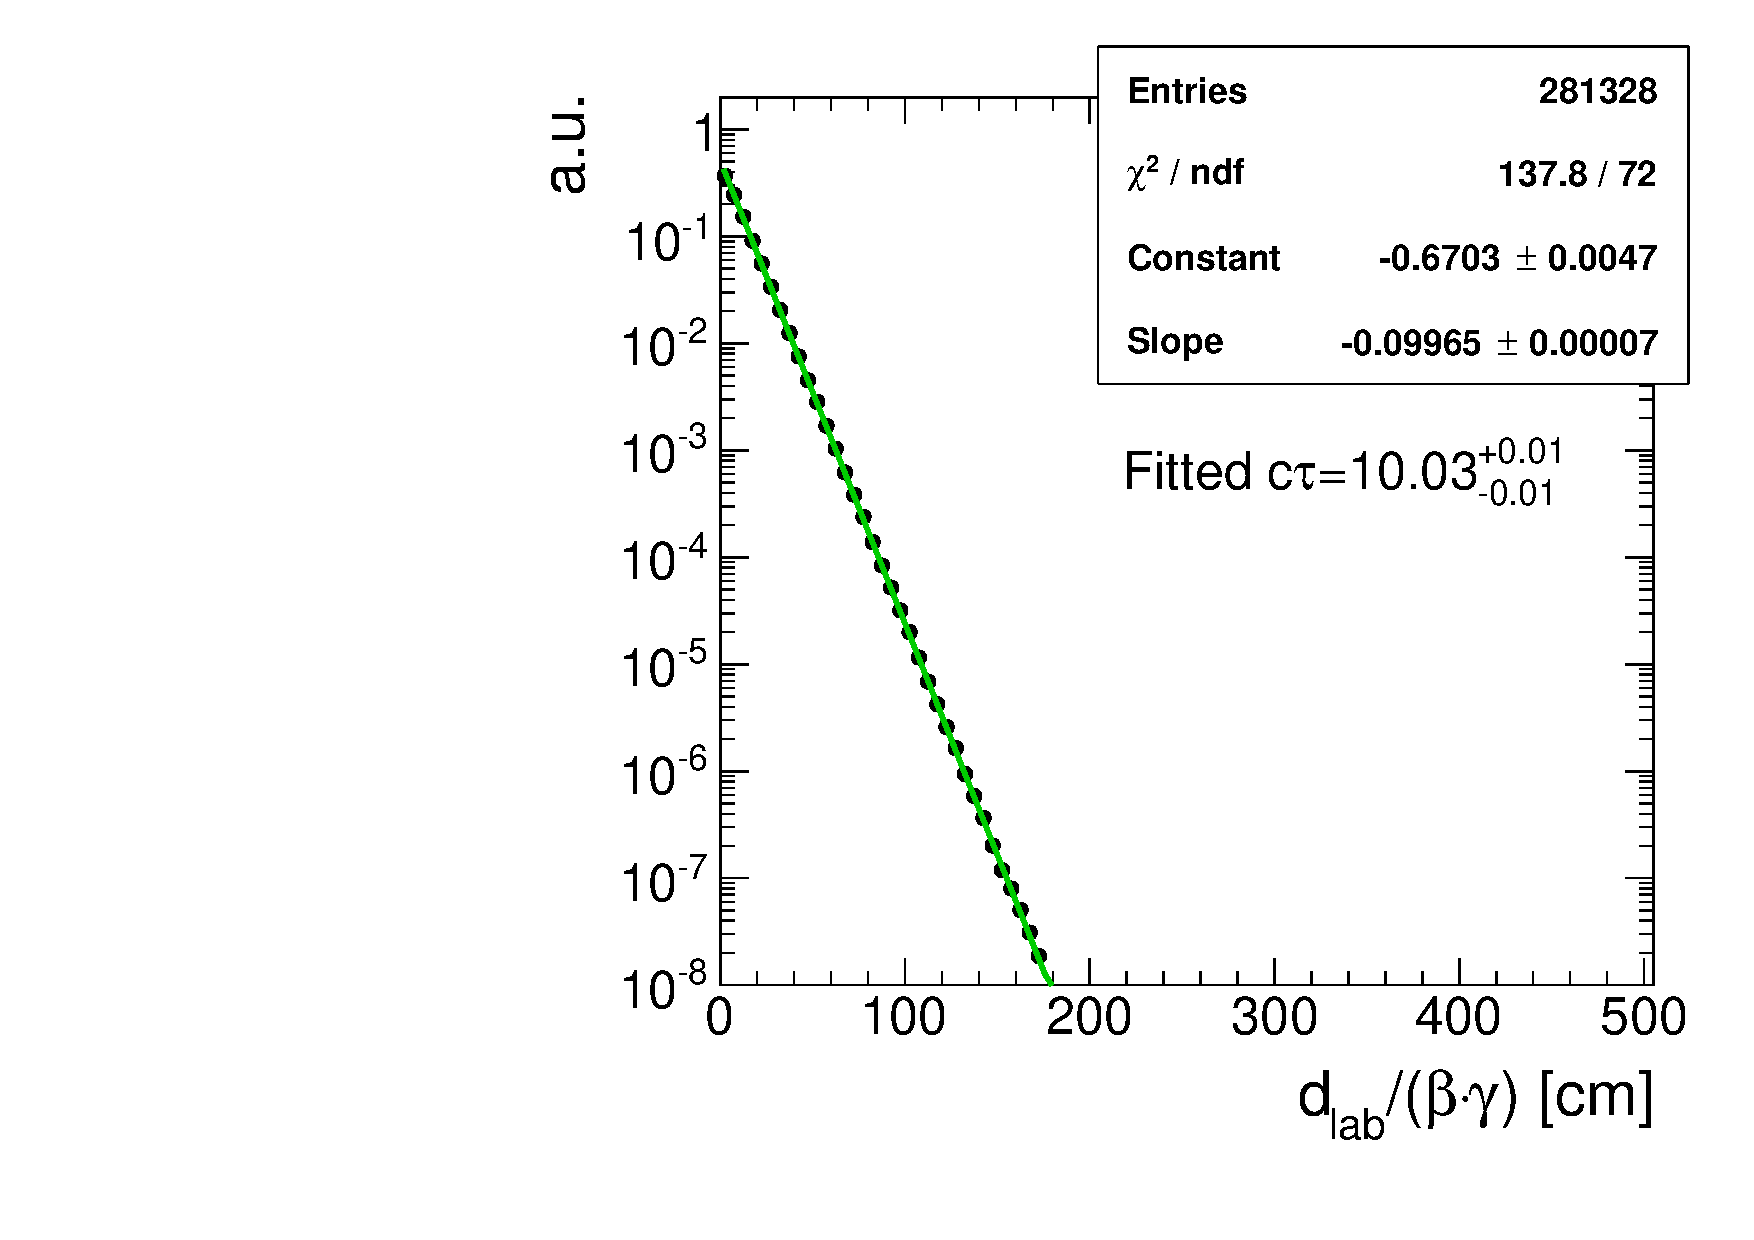
\includegraphics[width=0.49\textwidth]{figures/analysis/10cm.pdf}
  \end{tabular}
  \caption{Normalised distribution of the proper individual lifetime $d_{\text{lab}}/\left(\beta\gamma \right)$ of all charginos contained in a signal sample with a generated lifetime of $c\tau^{\text{gen}}=50\cm$ reweighted to a lifetime of $c\tau^{\text{target}}=10\cm$. Fitting an exponential curve $a\cdot \exp\left[\frac{1}{c \tau } c t_i\right]$ yields $c\tau=1./\text{Slope}=10\cm$.}
  \label{fig:LifetimeReweighting}
\end{figure}
It can be seen that the reweighting procedure does indeed reproduce the targeted lifetime of 10\cm.


All samples are generated for different masses of the chargino, but always almost mass-degenerate to the lightest neutralino.
The mass gap between chargino and neutralino is set to 150\mev.
However, as this analysis does not make use of the decay products of the chargino and the lifetime is independently set within \geant, the mass gap does not play any role.
Six different masses from 100\gev to 600\gev are simulated.
This leads to a total number of 42 signal samples.
In Table~\ref{tab:SignalCrossSections} cross sections at $\sqrt{s}=8\tev$ for $\chipm\chimp$ and $\chipm\chiO$ production 
for wino-like charginos and neutralinos are listed \cite{bib:SignalCrossSection_2012,bib:SignalCrossSection_2013}.
The cross section does not depend on the lifetime of the chargino.
\renewcommand{\arraystretch}{1.5}
\begin{table}[h]
\centering
\caption{Simulated signal mass points with corresponding cross sections at NLO-NLL (NLO: next-to-leading order, NLL: next-to-leading logarithmic) accuracy for wino-like charginos.}
\label{tab:SignalCrossSections}
\makebox[0.99\textwidth]{
\begin{tabular}{lll}
\multicolumn{3}{c}{} \\
\toprule
 $m_{\chipm}\left[\gev\right]$ & $\sigma_{\chipm\chimp}\left[\pb\right]$  & $\sigma_{\chiO\chimp}\left[\pb\right]$ \\
\midrule
 100     &  5.8234     &  11.5132 \\
 200     &  0.37924    &  0.77661 \\
 300     &  0.06751    &  0.14176 \\
 400     &  0.01751    &  0.03758 \\
 500     &  0.00553    &  0.01205 \\
 600     &  0.00196    &  0.00431 \\
\bottomrule
\end{tabular}}
\end{table}  

%%%%%%%%%%%%%%%%%%%%%%%%%%%%%%%%%%%%%%%%%%%%%%%%%%%%%%%%%%%%%%%%%%%%%%%%%%%%%%%%%%%%%%%%%%%%%%%%%%%%%%%%%%%%%%%%%%%%%%%%%%%%%%%%%%%%%%%%%%%%%%%%%%%%%%%%%%%%%%%%%%%%%%%%%%%%%%%%%%%%
%%%%%%%%%%%%%%%%%%%%%%%%%%%%%%%%%%%%%%%%%%%%%%%%%%%%%%%%%%%%%%%%%%%%%%%%%%%%%%%%%%%%%%%%%%%%%%%%%%%%%%%%%%%%%%%%%%%%%%%%%%%%%%%%%%%%%%%%%%%%%%%%%%%%%%%%%%%%%%%%%%%%%%%%%%%%%%%%%%%%
%%%%%%%%%%%%%%%%%%%%%%%%%%%%%%%%%%%%%%%%%%%%%%%%%%%%%%%%%%%%%%%%%%%%%%%%%%%%%%%%%%%%%%%%%%%%%%%%%%%%%%%%%%%%%%%%%%%%%%%%%%%%%%%%%%%%%%%%%%%%%%%%%%%%%%%%%%%%%%%%%%%%%%%%%%%%%%%%%%%%
\chapter{Event selection}
\label{sec:EventSelection}
\section{Datasets and triggers}
\label{sec:DatasetsAndTriggers}

The analysis is performed on pp collision data recorded in the year 2012 at the CMS experiment for a centre-of-mass energy of $\sqrt{s}=8\tev$.
In total an integrated luminosity of 19.7\fbinv was recorded in 2012.

As outlined in Section~\ref{sec:GeneralSearchStrategy}, the detection of chargino tracks is a challenging task already on trigger level.
Direct triggering of events containing chargino-like tracks is not possible because in 2012 there was no information about the tracking system available on trigger level L1.
Furthermore, there is no intrinsic missing transverse energy in the event if the chargino decays inside the tracker.
Therefore, this analysis uses initial state radiation for the detection of chargino events.
If ISR occurs, it is possible to trigger on a high-\pt jet (\ptfirstjet) and missing transverse energy (\met).

For this purpose, several triggers are utilised in this analysis.
An event is selected, if at least one of the three triggers in Table~\ref{tab:triggers} fired.
%
%To consider the event in the analysis, at least one of them must have fired.
%In Table~\ref{tab:triggers} the three triggers are listed together with the corresponding recorded integrated luminosity in the time when they were active.
\renewcommand{\arraystretch}{1.5}
\begin{table}[!hbt]
\centering
\caption{\met and \met+ jet triggers used in this analysis together with the corresponding recorded integrated luminosity during the time when they were in place.}
\label{tab:triggers}
\makebox[0.99\textwidth]{
\begin{tabular}{lr}
\multicolumn{2}{c}{} \\
\toprule
Trigger  & Luminosity [\fbinv]   \\
\midrule
 HLTMonoCentralPFJet80\_PFMETnoMu95\_NHEF0p95     &  5.3   \\
 HLTMonoCentralPFJet80\_PFMETnoMu105\_NHEF0p95    &  14.4  \\
 HLT\_MET120\_HBHENoiseCleaned                    &  19.7  \\
\bottomrule
\end{tabular}}
\end{table}  

The HLTMonoCentralPFJet80\_PFMETnoMu95\_NHEF0p95 and HLTMonoCentralPFJet80\_PFMETnoMu105\_NHEF0p95 triggers both rely on the L1 ETM40 trigger which requires the missing energy to be larger than 40\gev.
On HLT level, they further require at least one particle-flow jet with $\pt>80\gev$ and a missing transverse momentum (not taking into account the \pt of muons) to be larger than 95\gev or 105\gev respectively.
Finally, the energy release by neutral hadrons must not be larger than 95\% for all jets in the event.
The HLTMonoCentralPFJet80\_PFMETnoMu95\_NHEF0p95 trigger was active during Run\,A and Run\,B in 2012 data taking, whereas HLTMonoCentralPFJet80\_PFMETnoMu105\_NHEF0p95 was in place during Run\,C and Run\,D in 2012.

The HLT\_MET120\_HBHENoiseCleaned trigger is based on the two L1 triggers ETM40 and ETM36 that are combined by a logical OR.
On HLT level, the trigger requires that the missing energy measured in the calorimeter is larger than 120\gev.
The HBHENoise-filter reduces background from electronic noise in the HCAL.

The events that were selected by the described triggers are available in the datasets listed in Table~\ref{tab:SearchSamples}.
\renewcommand{\arraystretch}{1.5}
\begin{table}[!hbt]
\centering
\caption{MET data samples used in the search with the contained integrated luminosity.}
\label{tab:SearchSamples}
\makebox[0.99\textwidth]{
\begin{tabular}{lr}
\multicolumn{2}{c}{} \\
\toprule
Dataset  & Luminosity [\fbinv]   \\
\midrule
 /MET/Run2012A-22Jan2013-v1/RECO         &  0.876   \\
 /MET/Run2012B-22Jan2013-v1/RECO         &  4.412  \\
 /MET/Run2012C-22Jan2013-v1/RECO         &  7.055  \\
 /METParked/Run2012D-22Jan2013-v1/RECO   &  7.354  \\ 
\bottomrule
\end{tabular}}
\end{table}  
Again, because of the size of the datasets ($\sim150\,$TB in total), a reduction of the size is achieved by selecting only events where one of the used triggers fired and that contain at least one jet with a minimum \pt of 50\gev.\\

%In addition, the analysis makes use of the datasets listed in Table~\ref{tab:ControlSamples}.
%These datasets are used for background estimation purposes and the estimation of their associated systematic uncertainties.
%\renewcommand{\arraystretch}{1.5}
%\begin{table}[!hbt]
%\centering
%\caption{Further datasets used for background estimation.}
%\label{tab:ControlSamples}
%\makebox[0.99\textwidth]{
%\begin{tabular}{lr}
%\multicolumn{2}{c}{} \\
%\toprule
%Dataset  & Luminosity [\fbinv]   \\
%\midrule
%/SingleMu/Run2012A-22Jan2013-v1/AOD        &  0.876 \\
%/SingleMu/Run2012B-22Jan2013-v1/AOD        &  4.405 \\
%/SingleMu/Run2012C-22Jan2013-v1/AOD        &  7.040 \\
%/SingleMu/Run2012D-22Jan2013-v1/AOD        &  7.369 \\ 
%\midrule
%/SingleElectron/Run2012A-22Jan2013-v1/AOD  &  0.876 \\
%/SingleElectron/Run2012B-22Jan2013-v1/AOD  &  4.412 \\
%/SingleElectron/Run2012C-22Jan2013-v1/AOD  &  7.050 \\
%/SingleElectron/Run2012D-22Jan2013-v1/AOD  &  7.368 \\
%\bottomrule
%\end{tabular}}
%\end{table}  
%%%%%%%%%%%%%%%%%%%%%%%%%%%%%%%%%%%%%%%%%%%%%%%%%%%%%%%%%%%%%%%%%%%%%%%%%%%%%%%%%%%%%%%%%%%%%%%%%%%%%%%%%%%%%%%%%%%%%%%%%%%%%%%%%%%%%%%%%%%%%%%%%%%%%%%%%%%%%%%%%%%%%%%%%%%%%%%%%%%%
\section{Selection of signal candidate events}
\label{sec:AnalysisSelection}

In order to suppress events originating from Standard Model processes such as QCD-multijet events, \WJets, etc., a selection for signal-like tracks is applied.
The analysis selection closely follows the selection required in~\cite{bib:CMS:DT_Thesis,bib:CMS:DT_8TeV_AN}.
It relies on event-based and track-based variables as described in the following two sections.


\subsection{Event-based selection}
\label{sec:EventBasedSelection}
First a selection on the quality of the vertex is applied in order to suppress cosmic events and noise from the beam halo .
This selection includes requirements on the position of the vertex with respect to the beam axes and the number of degrees of freedom of the vertex which is strongly correlated to the number of tracks originating from the vertex~\cite{bib:CMS:Tracking_7TeV_PAS}:  
\begin{itemize}
\renewcommand{\labelitemi}{\footnotesize{\ding{118}}}
\item The vertex must have at least four degrees of freedom: \mbox{$vtx$ with $\geq 4$ d.o.f.}
\item The position of the vertex along the beam line must be within 24\cm with respect to the nominal interaction point: \mbox{$|dz| \leq 24\cm$.}
\item The position in the transverse direction must be within 2\cm with respect to the nominal interaction point: \mbox{$|d0| \leq 2\cm$.}
\end{itemize}
After these selection cuts are applied the remaining events are subjected to a further preselection.\\

To maximise the signal acceptance, the trigger related selection cuts are chosen as close as possible to the trigger thresholds (see Section~\ref{sec:DatasetsAndTriggers}).
In Fig.~\ref{fig:SignalMET+SignalJetPt}, the distributions of \met and the transverse momentum of the leading jet, \ptfirstjet, are shown for different signal models.
\begin{figure}[!t]
  \centering 
  \begin{tabular}{c}
    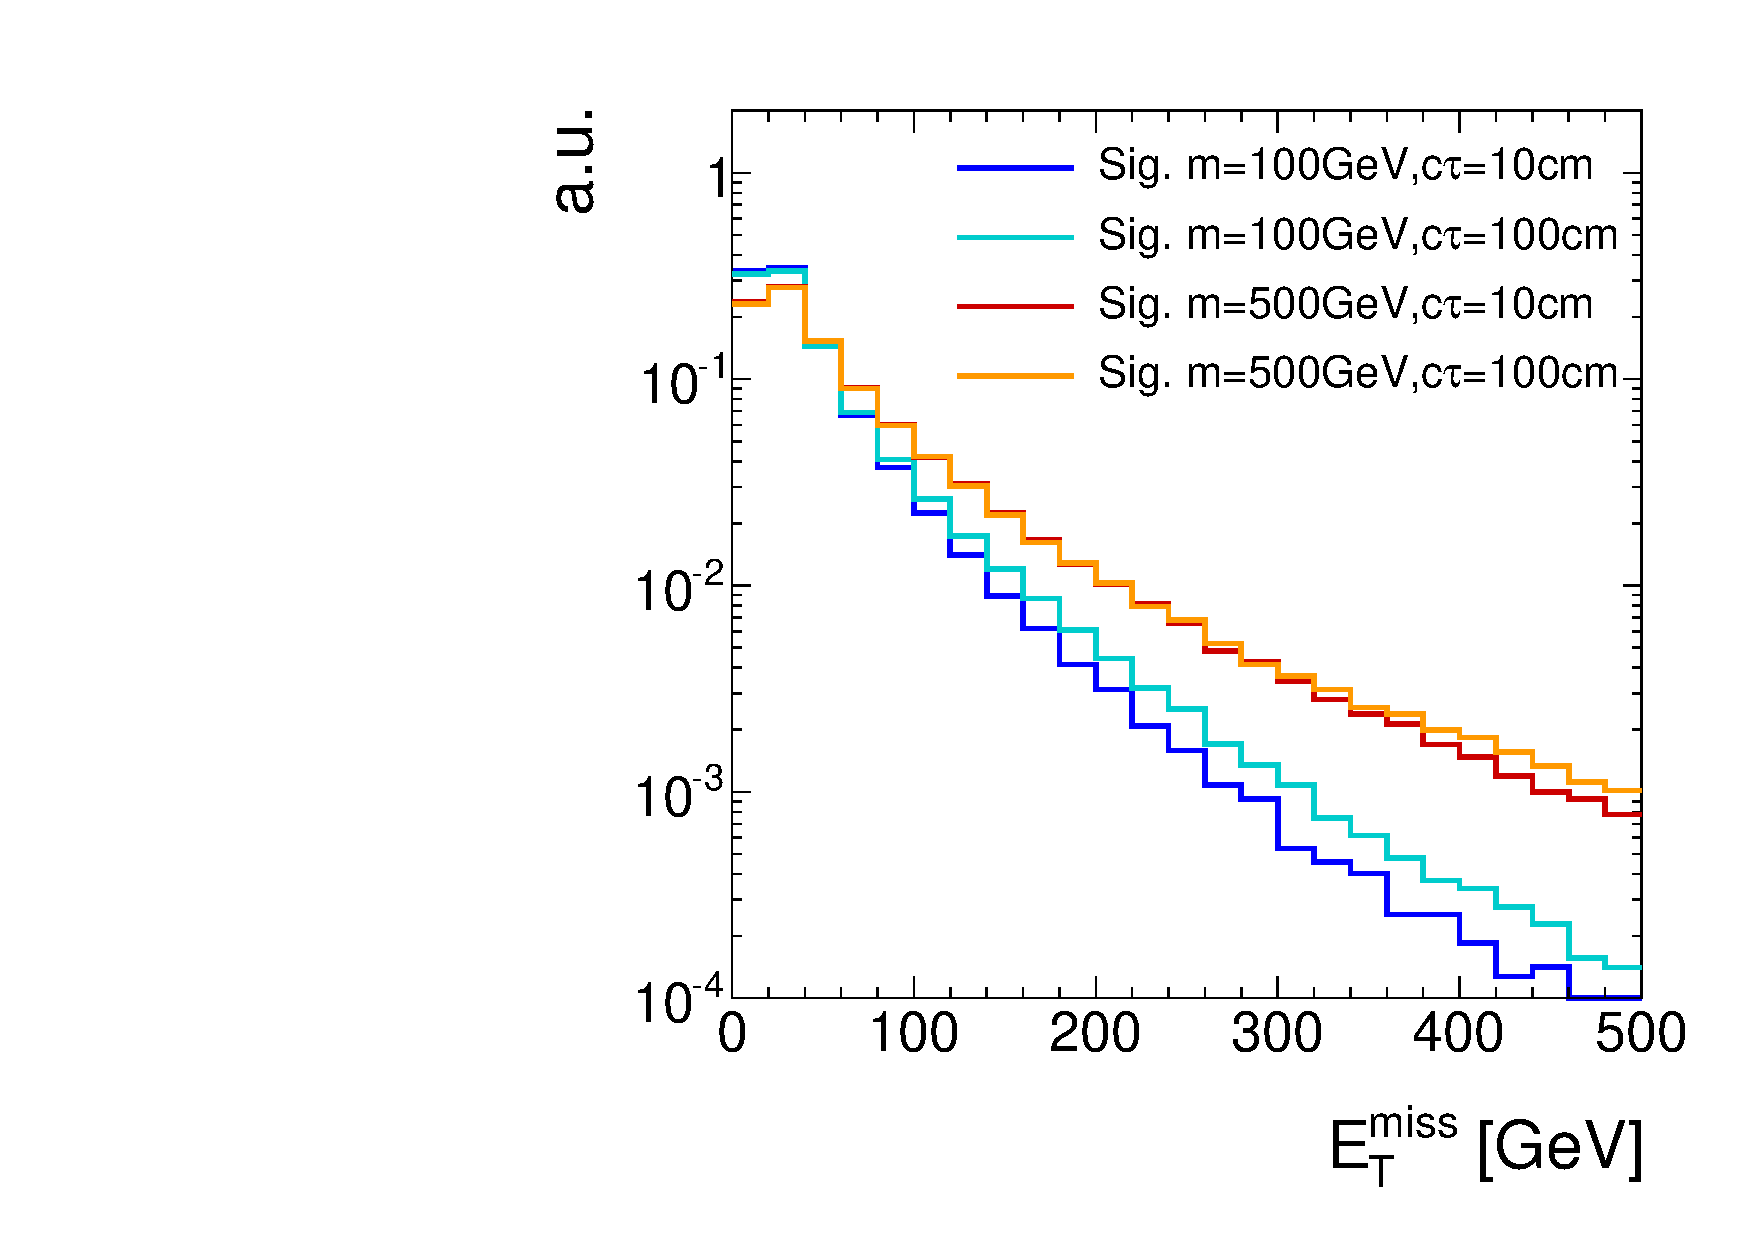
\includegraphics[width=0.49\textwidth]{figures/analysis/AnalysisSelection/hMetSmallRange_log_chiTracksnoSelection_4Signals.pdf}
    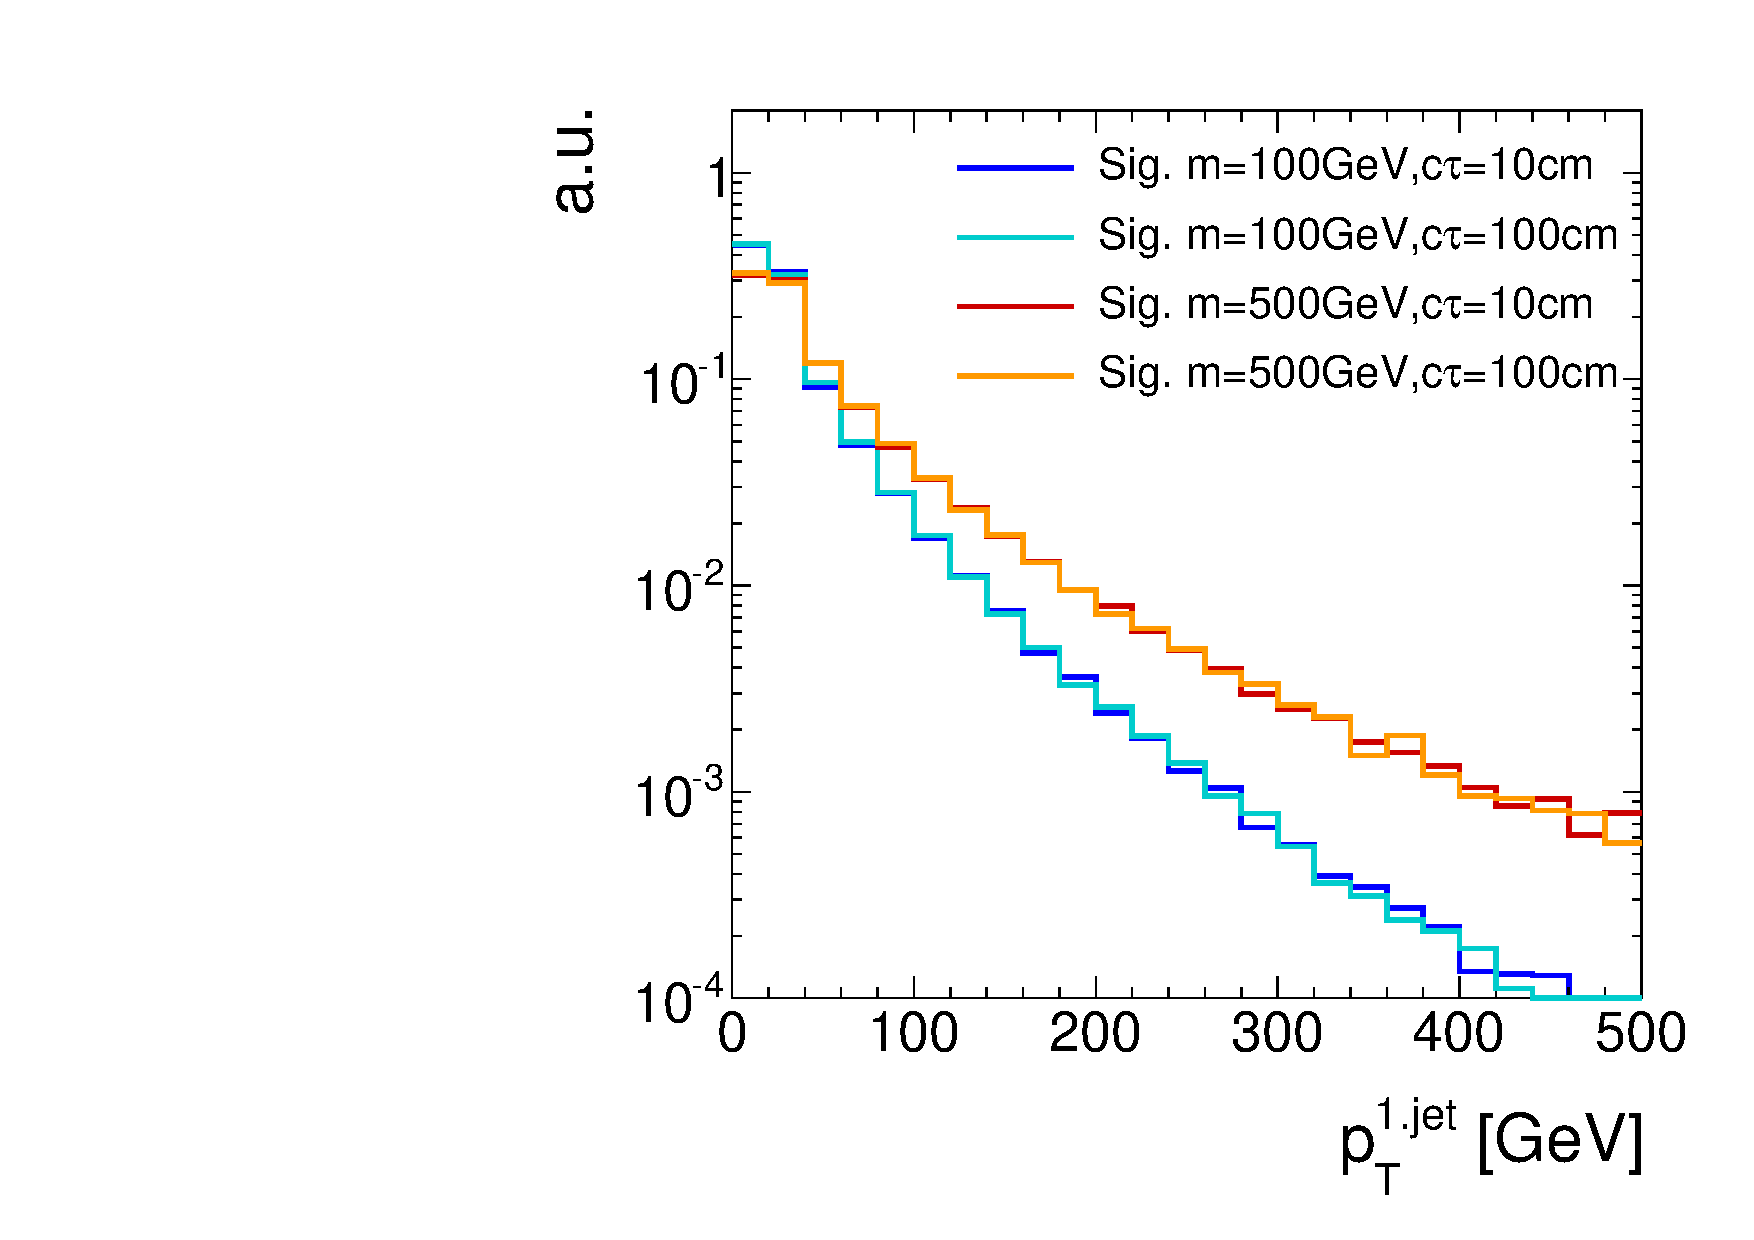
\includegraphics[width=0.49\textwidth]{figures/analysis/AnalysisSelection/h1stjetptSmallRange_log_chiTracksnoSelection_4Signals.pdf}
  \end{tabular}
  \caption{Normalised distributions of the missing transverse momentum (left) and the transverse momentum of the leading jet (right) for four different signal models.}
  \label{fig:SignalMET+SignalJetPt}
\end{figure}
Only jets with $|\eta|<2.4$ that fulfil the following further criteria are taken into account:
\begin{itemize}
\item Charged hadron energy fraction $>0.2$
\item Charged electromagnetic energy fraction $<0.5$
\item Neutral hadron energy fraction $<0.7$
\item Neutral electromagnetic energy fraction $<0.7$.
\end{itemize}
These additional jet quality criteria ensure that noise from cosmic and beam halo muons and high-\pt photons and electrons is suppressed \cite{bib:CMS:DM_8TeV_AN}.

The trigger efficiency as a function of \met and \ptfirstjet was determined within~\cite{bib:CMS:DM_8TeV} with a single-muon reference sample.
The trigger paths become fully efficient for \mbox{$\ptfirstjet \gtrsim 110\gev$} and \mbox{$\met \gtrsim 220\gev$~\cite{bib:CMS:DM_8TeV_AN}}.
However, it can be seen in Fig.~\ref{fig:SignalMET+SignalJetPt} that for a selection of \mbox{$\met>220\gev$} more than 99\% of the signal events are rejected.

In order to achieve a reasonable signal acceptance, this search imposes a trigger selection closer to the intrinsic trigger thresholds.
The trigger requirements are as follows:
\begin{itemize}
\renewcommand{\labelitemi}{\footnotesize{\ding{118}}}
\item There is at least one jet within $|\eta|<2.4$ with transverse momentum larger than 110\gev which fulfils the above mentioned jet noise cleaning criteria: \mbox{$\ptfirstjet>110\gev$}.
\item The missing transverse momentum must be larger than 100\gev: \mbox{$\met>100\gev$}
\end{itemize}
These requirements result in a trigger efficiency of 100\% in the variable \ptfirstjet and $\sim20\%$ in the variable \met at the cut thresholds~\cite{bib:CMS:DM_8TeV_AN}.\\

Because of the huge cross section, QCD-multijet events are frequently produced at the LHC.
Due to jet energy mismeasurements, they can also contribute to data samples recorded with MET triggers.
Therefore, special requirements are enforced in order to suppress events emerging from strong production processes.
QCD-multijet events can be characterised by topologies where two jets are almost back-to back.
Additionally, in QCD-multijet events the missing energy is usually aligned with one of the leading jets in the event.
Figure~\ref{fig:QCDcuts} shows the maximum $\Delta\phi$ of any of two jets and the minimum $\Delta\phi$ between the \met vector and any of the two leading jets for the SM background and two different signal datasets.

Therefore the following two requirements are sufficient to suppress QCD-multijet events efficiently:
\begin{itemize}
\renewcommand{\labelitemi}{\footnotesize{\ding{118}}}
\item $\Delta\phi$ between any of two jets (with $\pt>20\gev$ and $|\eta|<4.5$) in the event must be smaller than 2.5. %: \mbox{$\Delta\phi\left( j_i, j_j\right)<2.5$}.
\item $\Delta\phi$ between any of the two leading jets (with $\pt>20\gev$ and $|\eta|<4.5$) and the \met must be larger than 0.5. %: \mbox{$\Delta\phi\left( j_{1,2}, \metvec \right) > 0.5$.} 
\end{itemize}

\begin{figure}[!t]
  \centering 
  \begin{tabular}{c}
    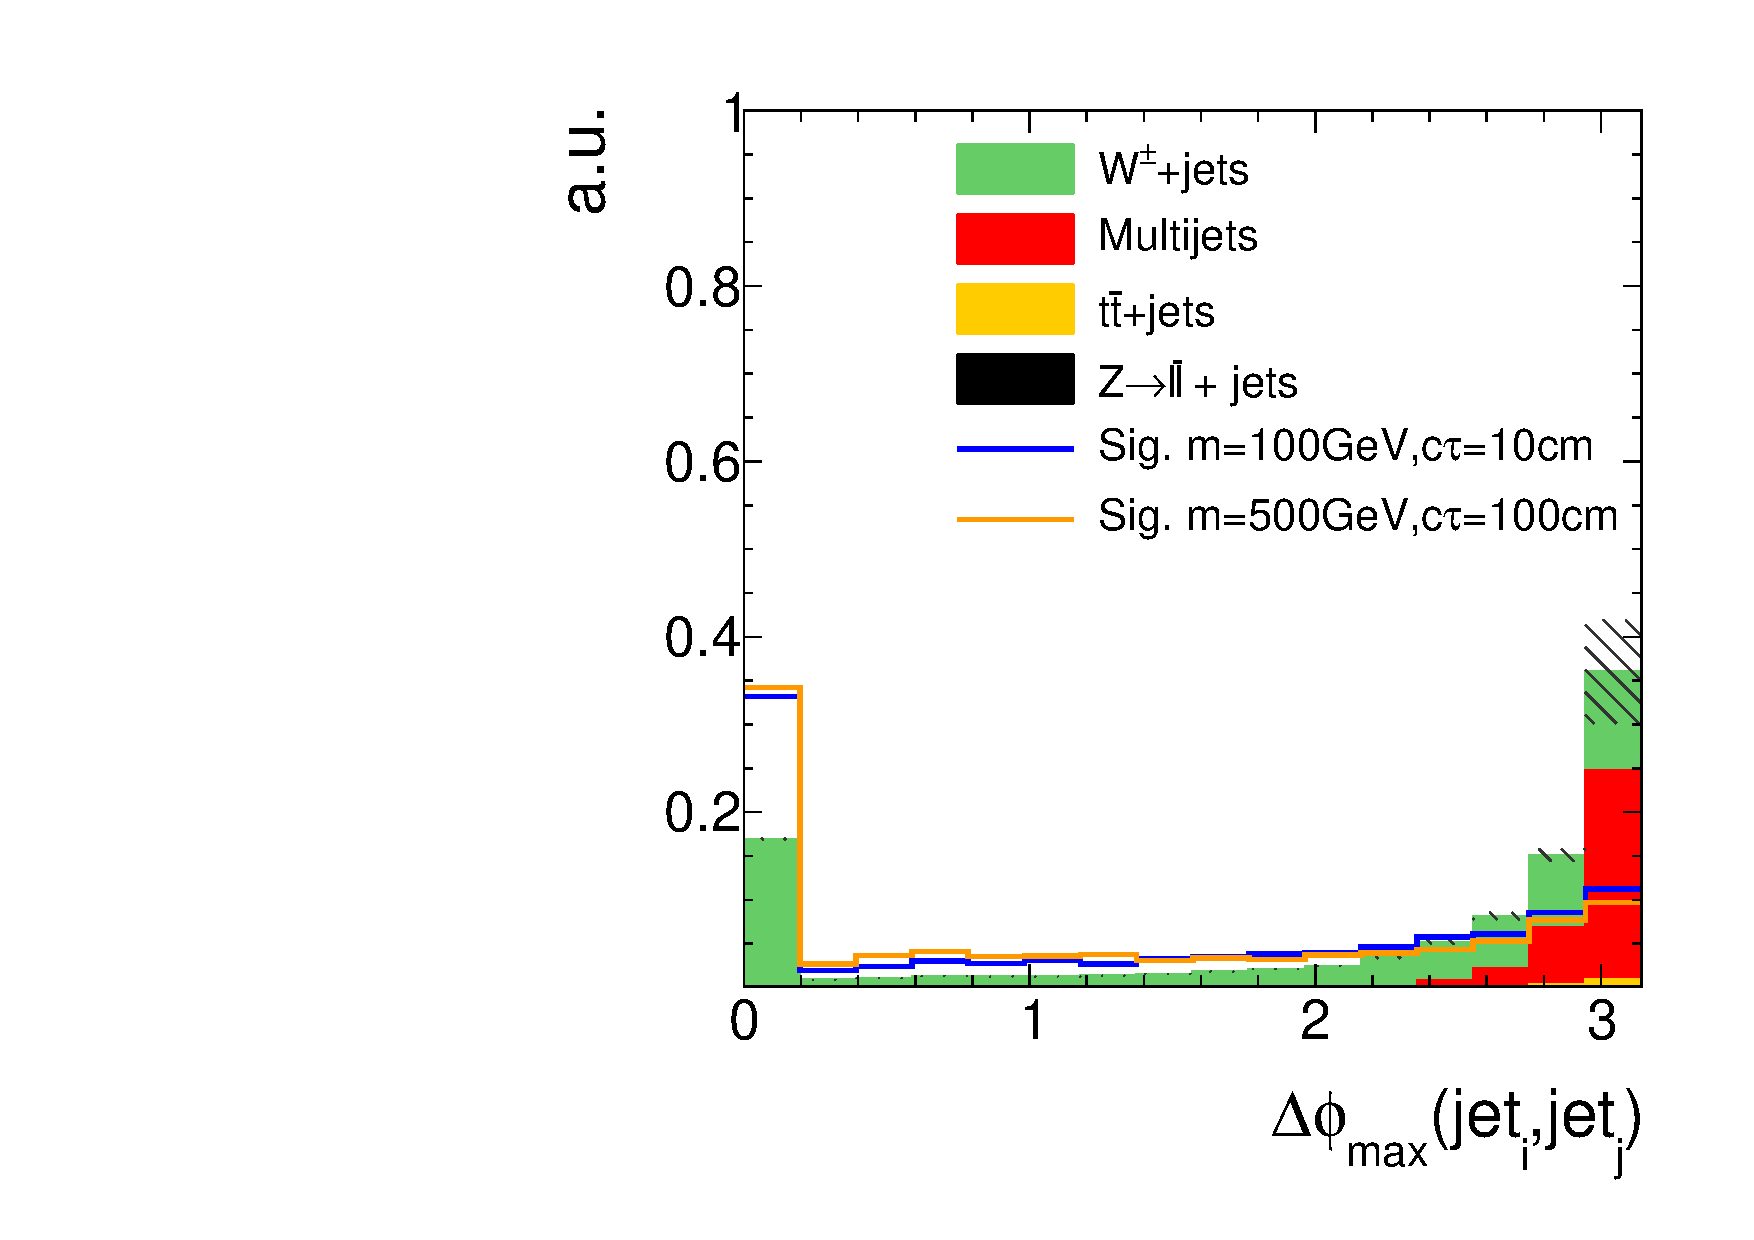
\includegraphics[width=0.49\textwidth]{figures/analysis/AnalysisSelection/chiTrackstriggerRequirementsTrigger_2Signals_FullBkg/hDeltaPhiMaxbeforeCut_lin.pdf}
    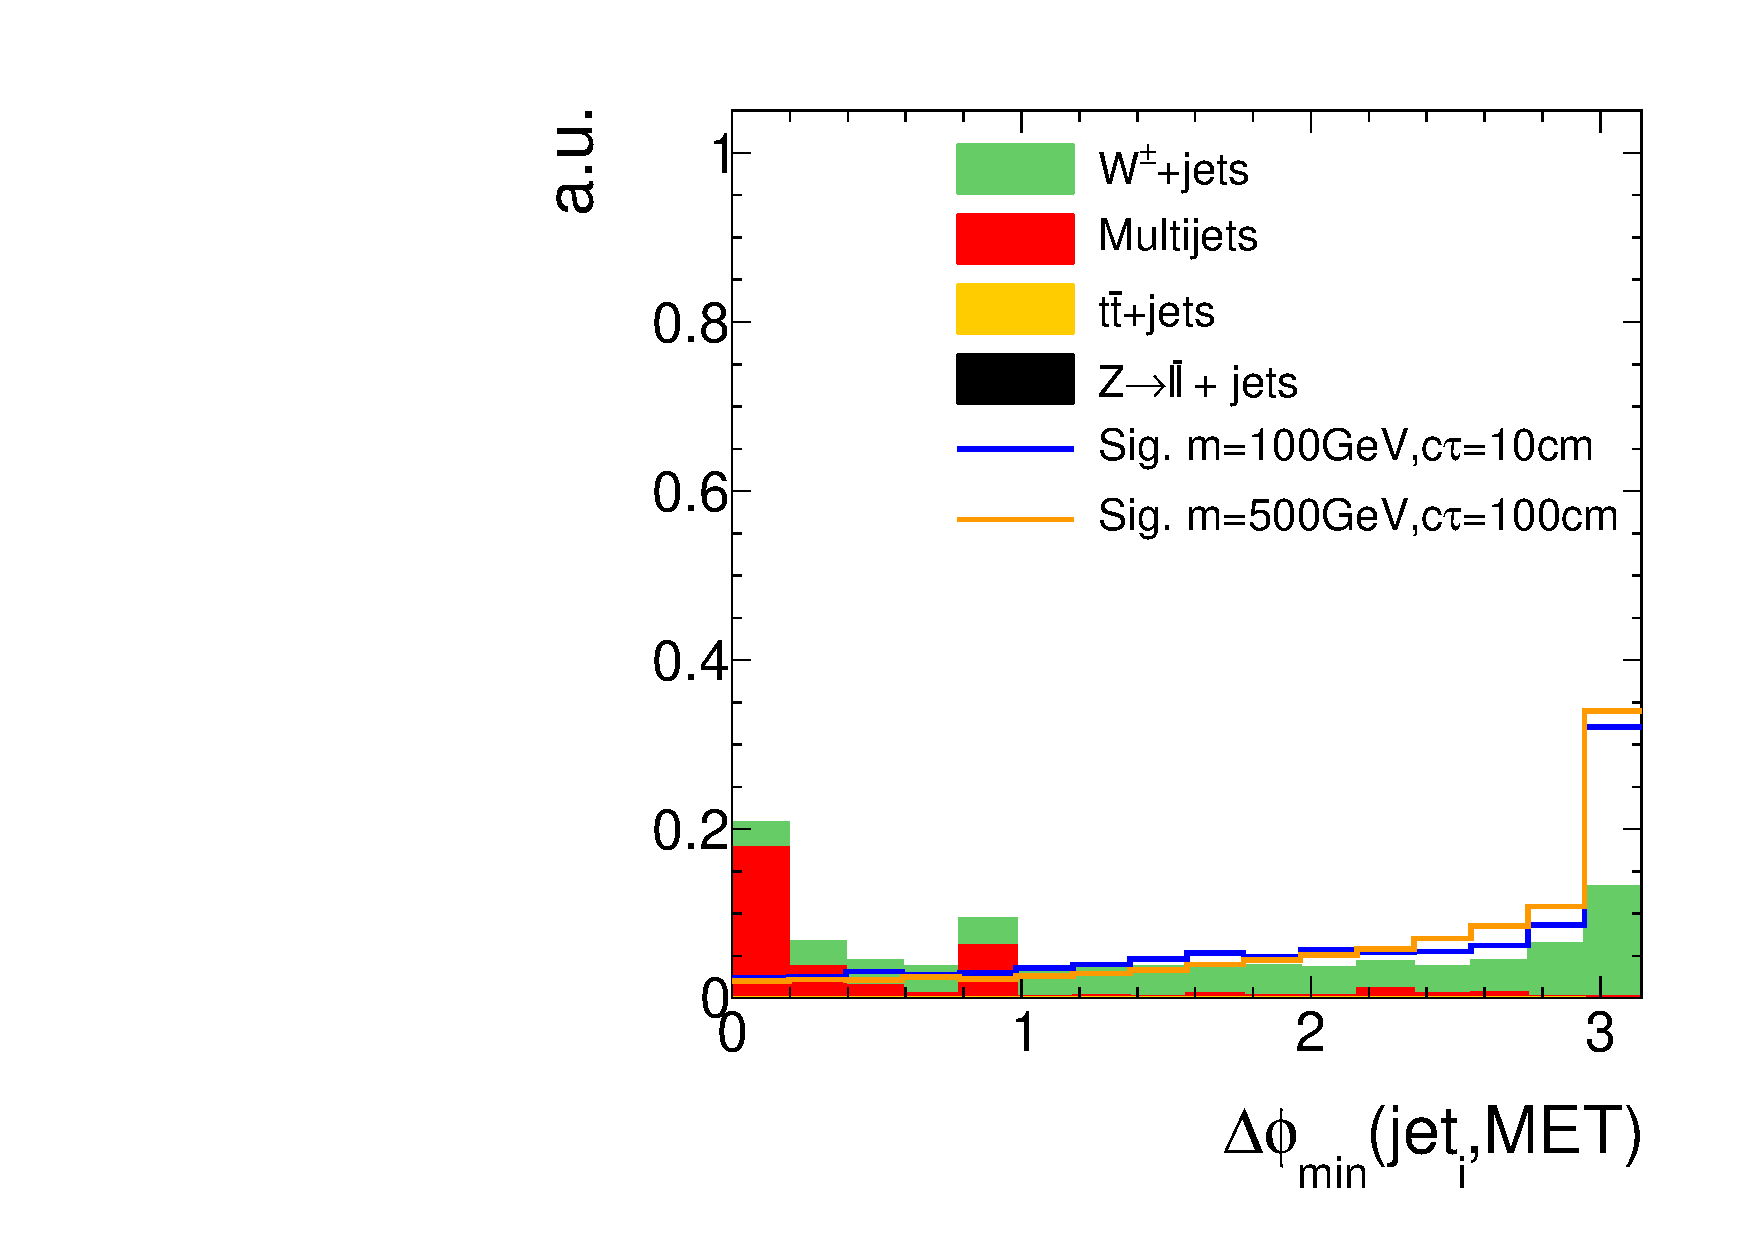
\includegraphics[width=0.49\textwidth]{figures/analysis/AnalysisSelection/chiTrackstriggerRequirementsTrigger_2Signals_FullBkg/hDeltaPhiJetMetMinbeforeCut_lin.pdf}
  \end{tabular}
  \caption{Maximum $\Delta \phi$ between any of two jets (left) and the minimum $\Delta \phi$  between the \met vector and any of the two leading jets (right) normalised to unit area after the trigger selection.
           Only jets with $\pt>20\gev$ and $|\eta|<4.5$ are considered.}
  \label{fig:QCDcuts}
\end{figure}
\hspace{0.9cm}

\subsection{Candidate track selection}
\label{sec:CandidateTrackSelection}
After the reduction of background processes with event-based variables, a track-based selection is carried out.
To get an optimised selection for possible chargino tracks several signal track characteristics are exploited.\\

First, a selection of high quality tracks is enforced:
\begin{itemize}
\renewcommand{\labelitemi}{\footnotesize{\ding{118}}}
\item The track must be of ``high purity'' as defined in~\cite{bib:CMS:Tracking_2010}.
\item The track is required to have no missing middle or inner hits: $N_{\text{miss}}^{\text{middle/inner}}=0$
\item The radial and longitudinal  distance of the track to the primary vertex must be small: \mbox{$|d0|<0.02\cm$}, \mbox{$|dz|<0.5\cm$}.
\end{itemize}
In Figs.~\ref{fig:LostHits} and~\ref{fig:d0_dz}, the power of the latter two quality selection cuts is shown.\\
\begin{figure}[!b]
  \centering 
  \begin{tabular}{c}
    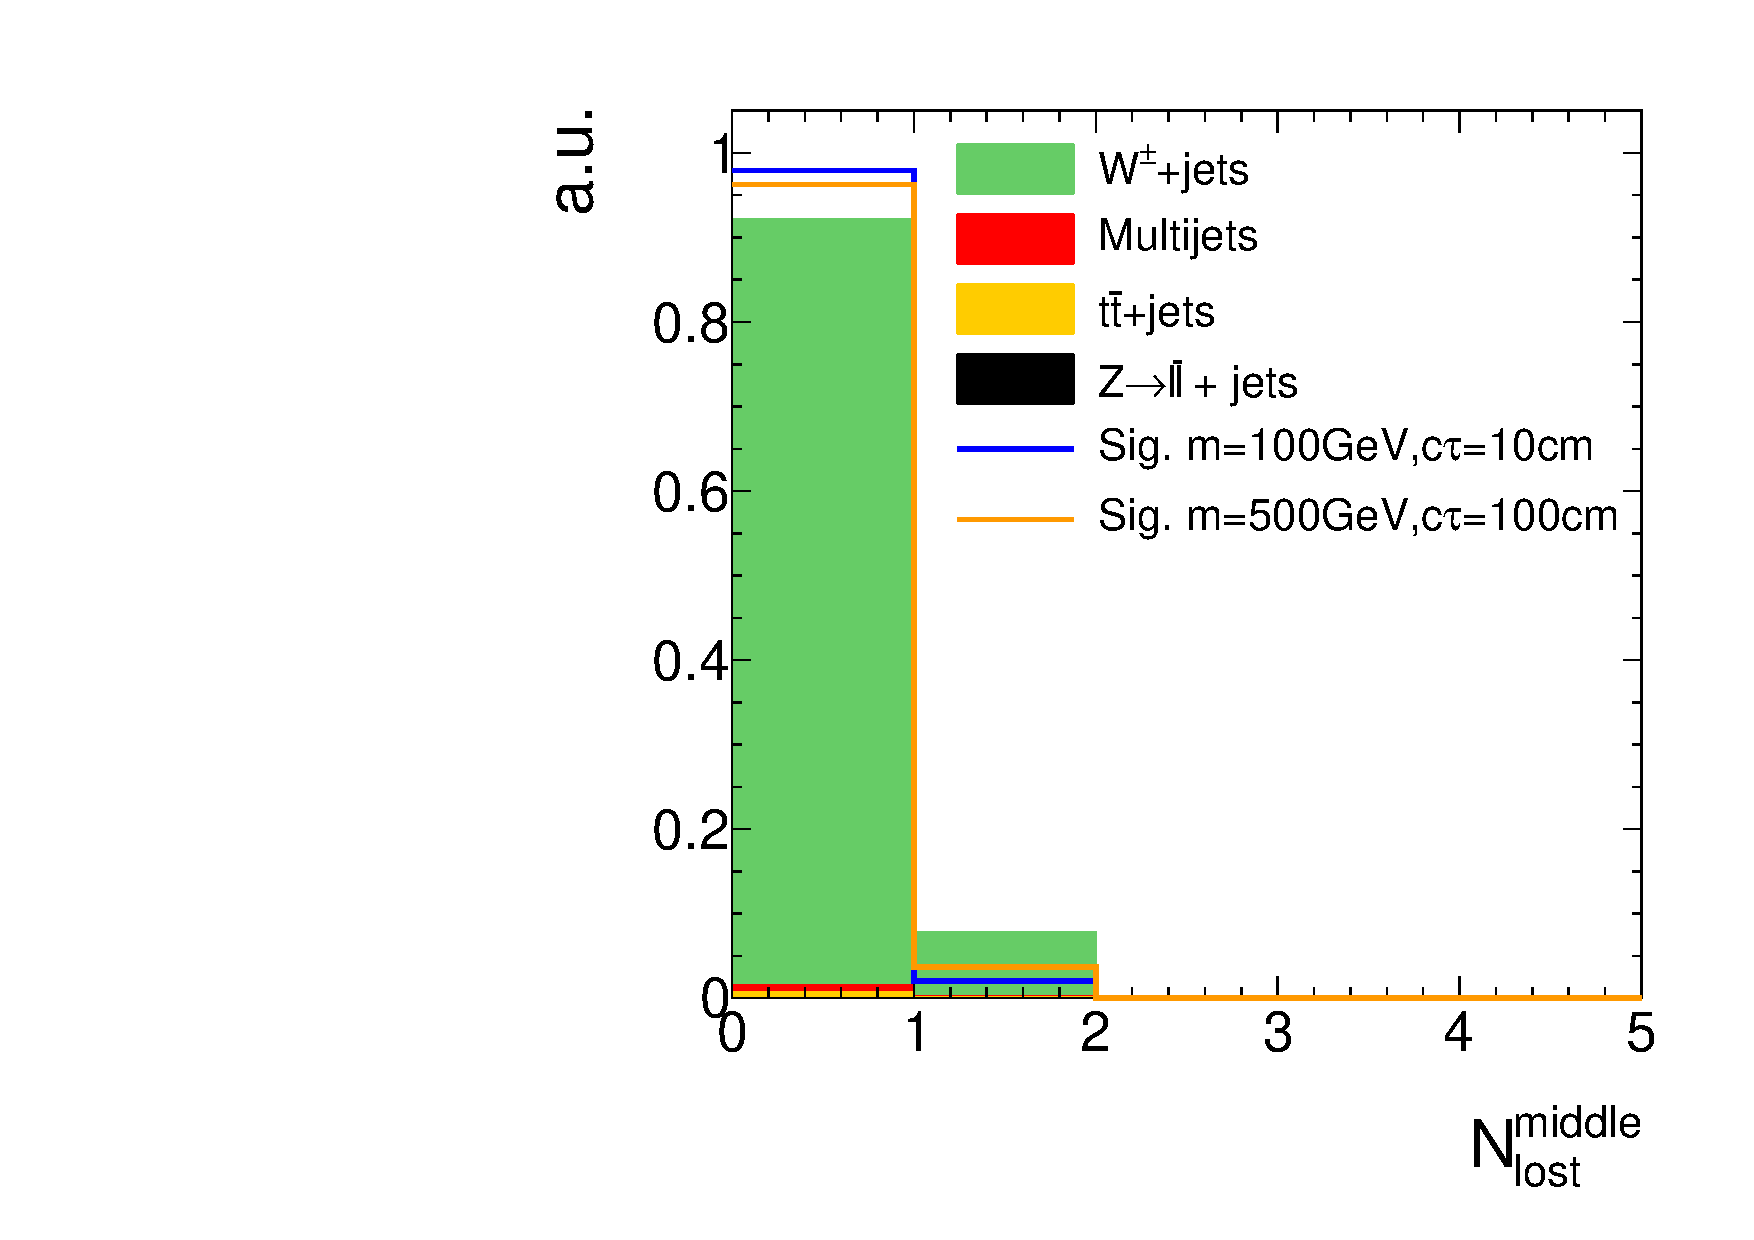
\includegraphics[width=0.49\textwidth]{figures/analysis/AnalysisSelection/chiTracksQCDsupressionTrigger_2Signals_FullBkg/htrackNLostMid_lin.pdf}
    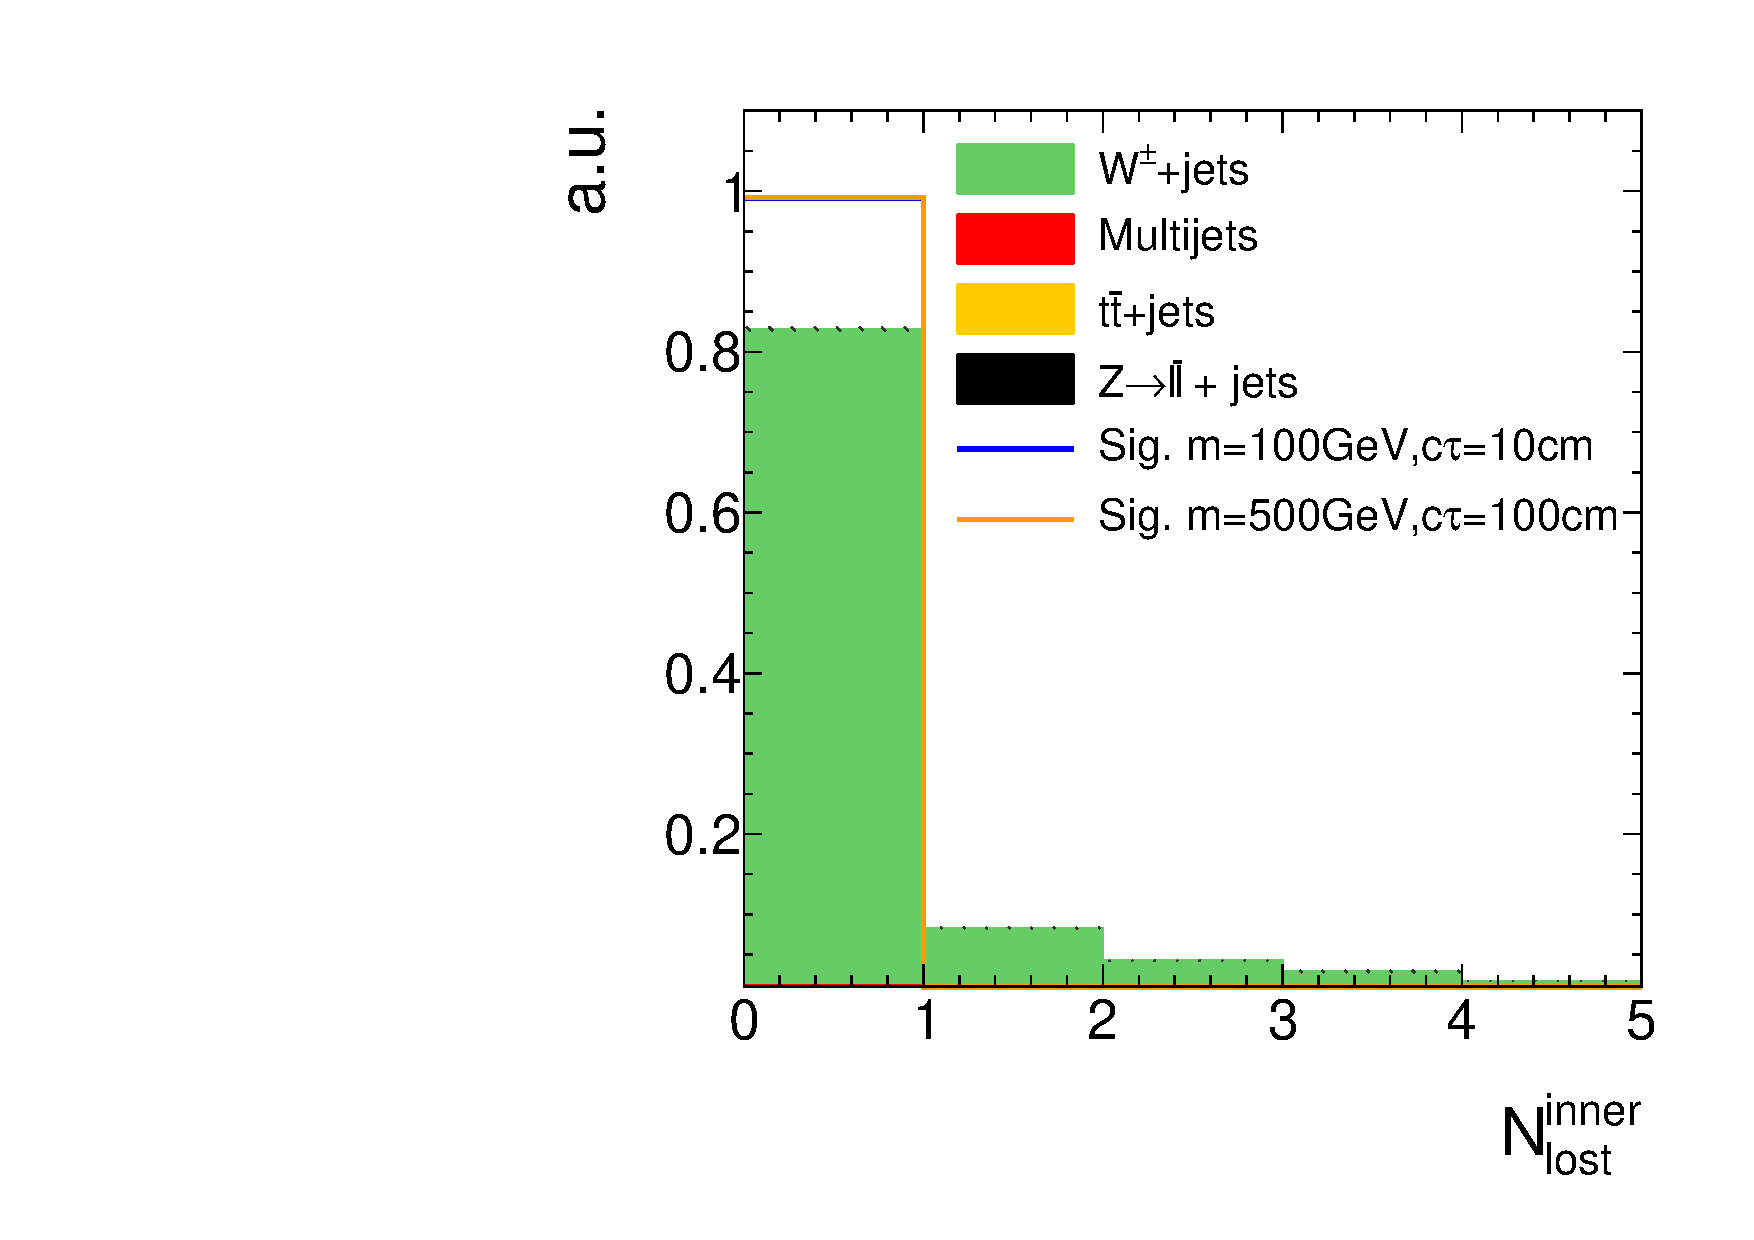
\includegraphics[width=0.49\textwidth]{figures/analysis/AnalysisSelection/chiTracksQCDsupressionTrigger_2Signals_FullBkg/htrackNLostInner_lin.pdf}
  \end{tabular}
  \caption{Number of missing middle (left) and inner (right) hits of background and signal tracks after trigger requirements and QCD suppression cuts.}
  \label{fig:LostHits}
\end{figure}
\begin{figure}[!t]
  \centering 
  \begin{tabular}{c}
    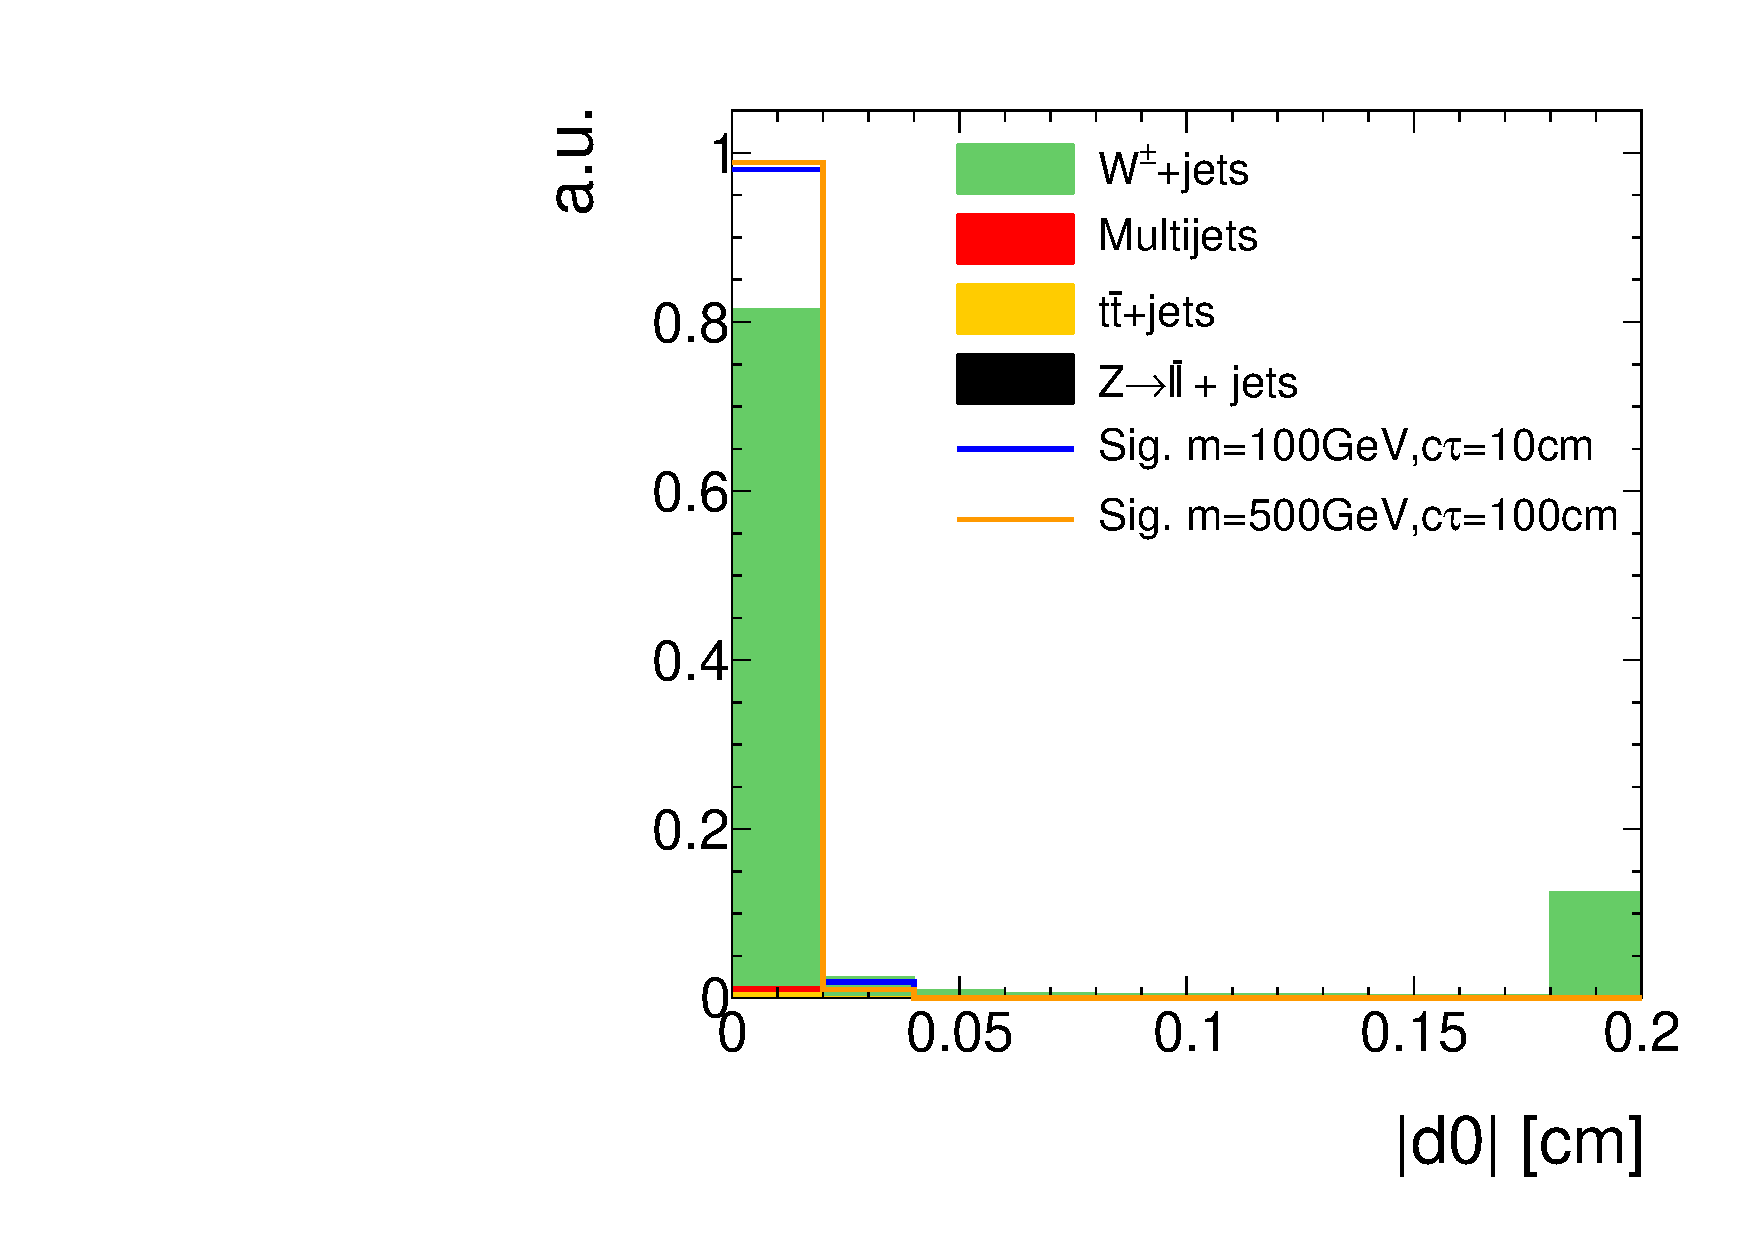
\includegraphics[width=0.49\textwidth]{figures/analysis/AnalysisSelection/chiTracksQCDsupressionTrigger_2Signals_FullBkg/htrackd0_lin.pdf}
    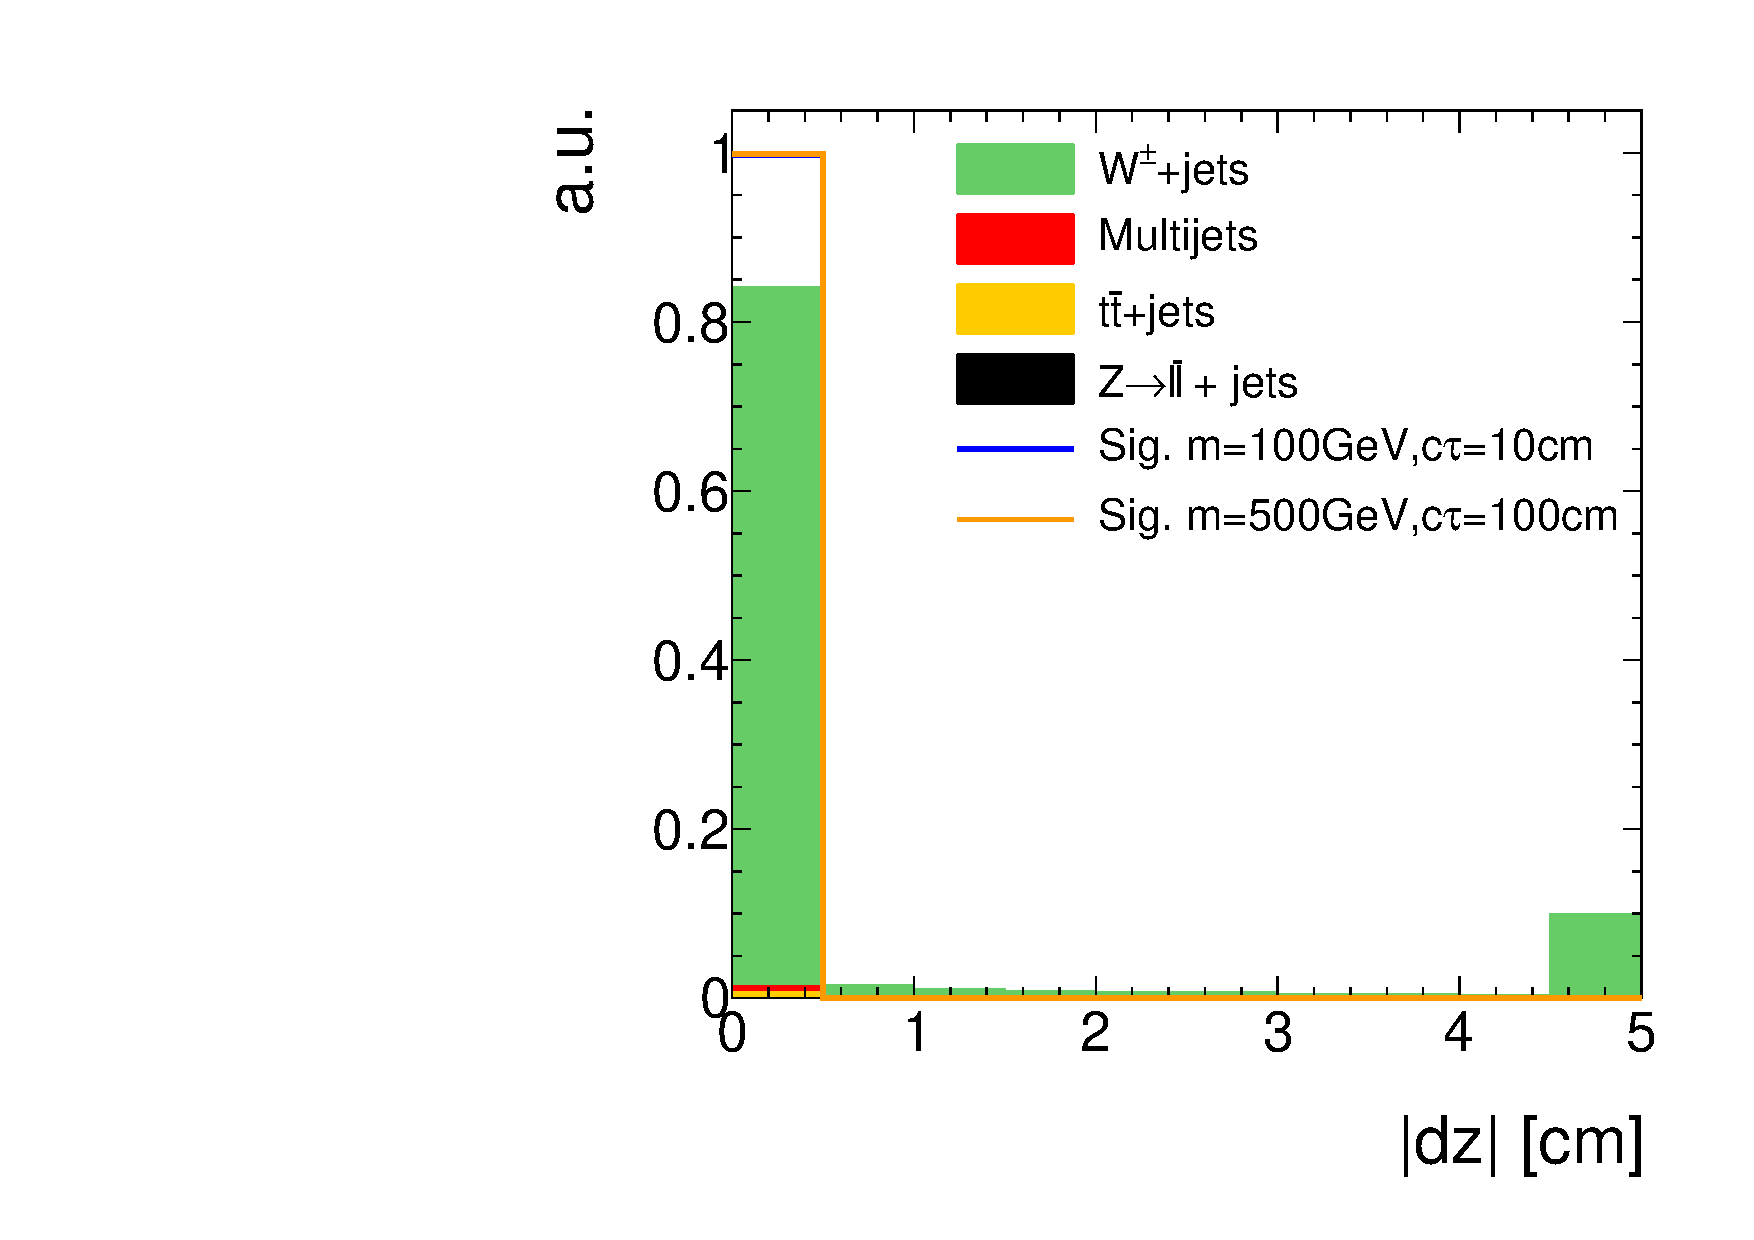
\includegraphics[width=0.49\textwidth]{figures/analysis/AnalysisSelection/chiTracksQCDsupressionTrigger_2Signals_FullBkg/htrackdz_lin.pdf}
  \end{tabular}
  \caption{Absolute value of the radial (left) and longitudinal (right) distance between the track and the primary vertex after trigger requirements and multijet suppression cuts. 
           Overflow entries are added to the last bin.}
  \label{fig:d0_dz}
\end{figure}

Furthermore, a first kinematic preselection is applied:
\begin{itemize}
\renewcommand{\labelitemi}{\footnotesize{\ding{118}}}
\item Only tracks in the central region are considered : $|\eta|<2.1$.
\item Only tracks with a minimum transverse momentum of 20\gev are considered: \mbox{$\pt>20\gev$}.\\
\end{itemize}
%\hspace{0.7cm}
%%%%%%%%%%%%%%%%%%%%%%%%%%%%%%%%%%%%%%%%%%%%%%%%%%%%%%%%%%%%%%%%%%%%%%%%

In order to suppress background tracks emerging from SM processes, an electron, muon and tau veto is applied.
This rejects tracks that are close to a reconstructed electron, muon or tau.
Additionally, the candidate track must not be close to a jet ($\pt>20\gev$ and $|\eta|<4.5$).

Unfortunately, the lepton veto selection cuts lack efficiency in some of the detector directions.
For example, the reconstruction of an electron easily fails in the direction of a dead ECAL cell.
This reduces the discrimination power of the electron veto.
For this reason, tracks that point towards dead or noisy ECAL cells are rejected.
A general list of dead and noisy ECAL cells is provided centrally at CMS.
Further dead cells were identified within a study in~\cite{bib:CMS:DT_Thesis,bib:CMS:DT_8TeV_AN} resulting in a total number of 1234 dead or noisy ECAL channels. 
These are illustrated in Fig.~\ref{fig:DeadECALmap} showing a map of all ECAL channels not considered in the search.


Additionally, tracks that point towards intermodule gaps of ECAL cells or to the ECAL barrel endcap gap at $1.42<|\eta|<1.65$ are rejected.
A list of the ECAL intermodule gaps, that is supplied centrally at CMS, is given in Table~\ref{tab:IntermoduleGaps}.

The muon reconstruction is less efficient for muons in detector regions with bad cathode strip chambers (CSC).
These bad chambers are also identified centrally at CMS and their $\eta$ and $\phi$ values are visualised in Fig.~\ref{fig:BadCSCMap}.
Thus, also tracks pointing towards these regions within a distance of $\Delta R<0.25$ are rejected.

\begin{figure}[!t]
  \centering 
  \begin{tabular}{c}
    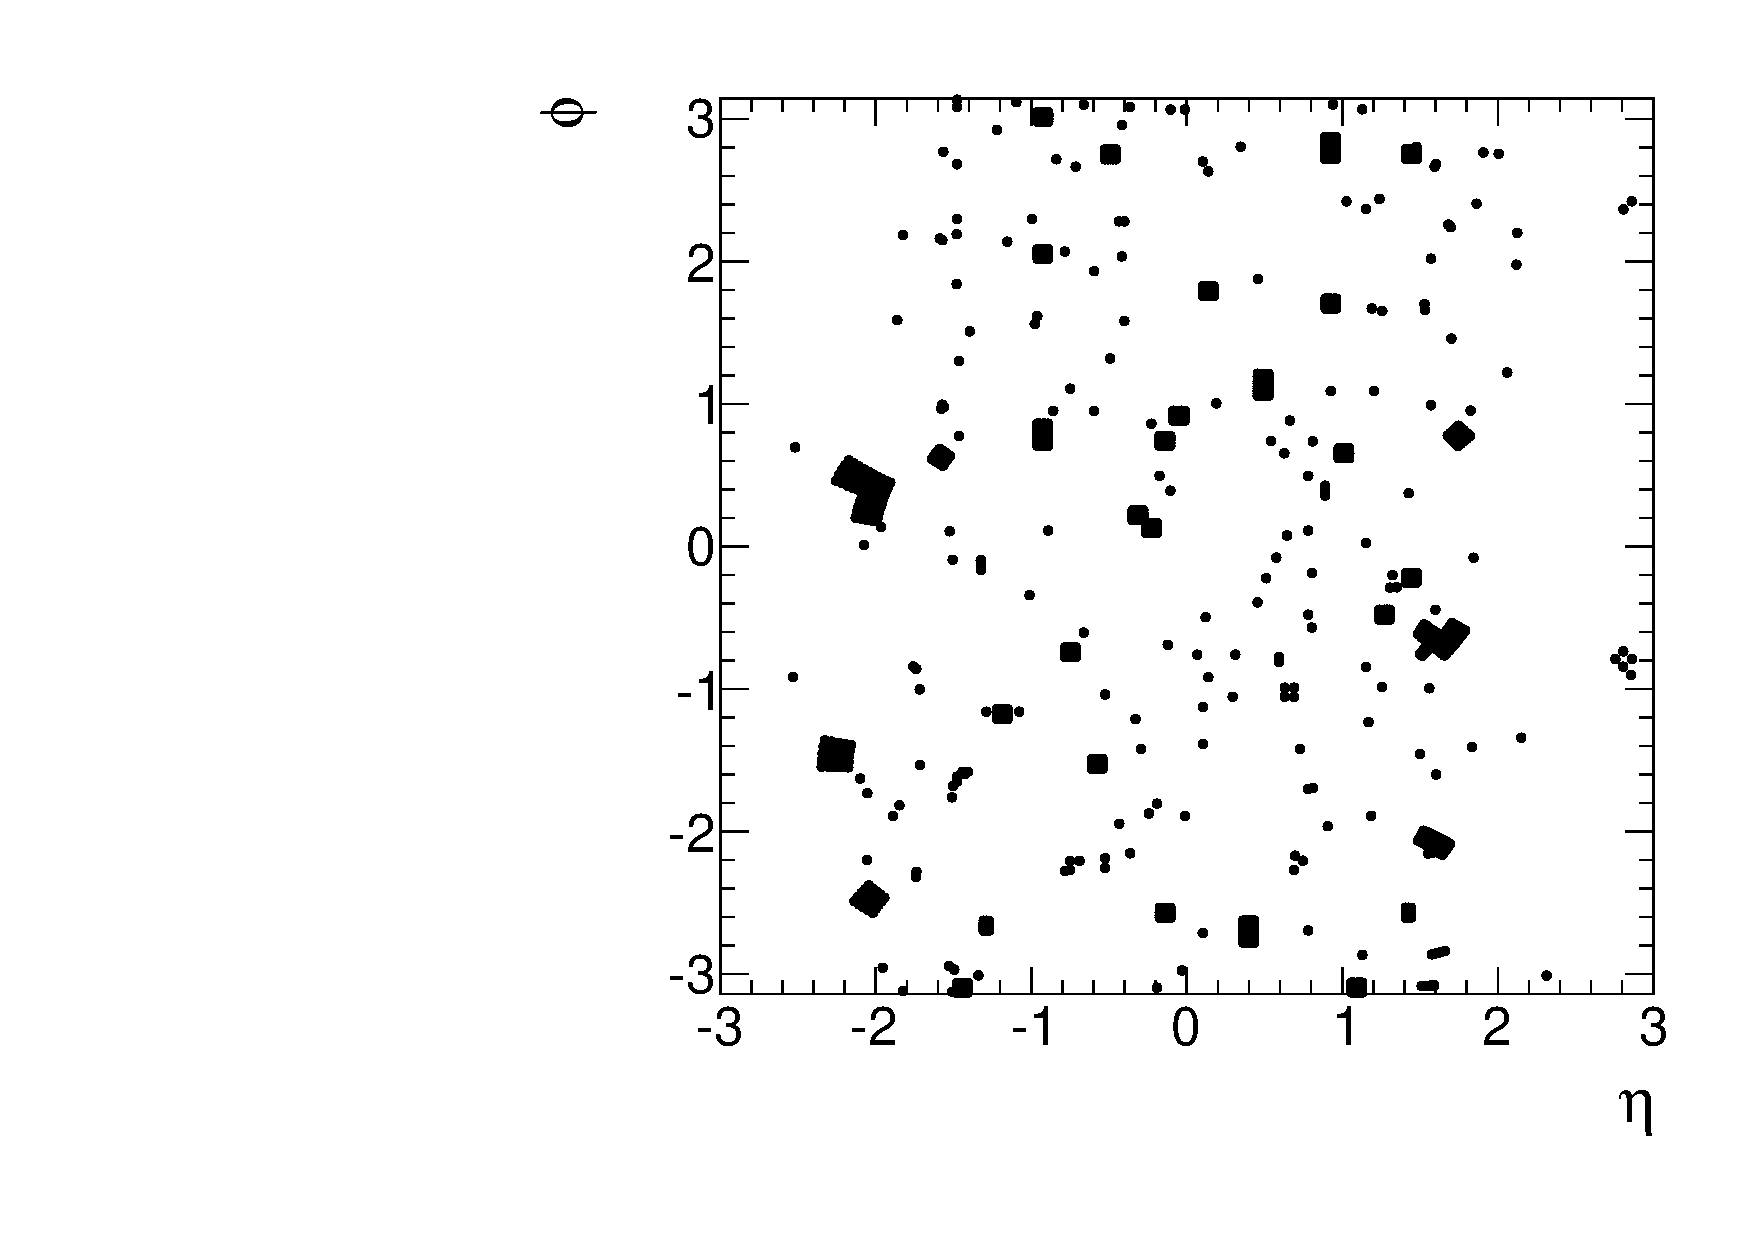
\includegraphics[width=0.49\textwidth]{figures/analysis/DeadECALMap.pdf}
  \end{tabular}
  \caption{Visualisation of dead and noisy ECAL cells in the detector's $\phi - \eta$ plane according to~\cite{bib:CMS:DT_Thesis,bib:CMS:DT_8TeV_AN}.}
  \label{fig:DeadECALmap}
\end{figure}

\renewcommand{\arraystretch}{1.5}
\begin{table}[!b]
\centering
\caption{Intermodule ECAL gaps.}
\label{tab:IntermoduleGaps}
\makebox[0.99\textwidth]{
\begin{tabular}{c}
\multicolumn{1}{c}{} \\
\toprule
$\eta$-ranges     \\
\midrule
 -1.14018  $< \eta <$ -1.1439 \\
-0.791884  $< \eta <$ -0.796051 \\
-0.44356   $< \eta <$  -0.447911 \\
0.00238527 $< \eta <$ -0.00330793 \\
0.446183   $< \eta <$ 0.441949 \\
0.793955   $< \eta <$ 0.789963 \\
1.14164    $< \eta <$ 1.13812 \\
\bottomrule
\end{tabular}}
\end{table}  

\begin{figure}[!t]
  \centering 
  \begin{tabular}{c}
    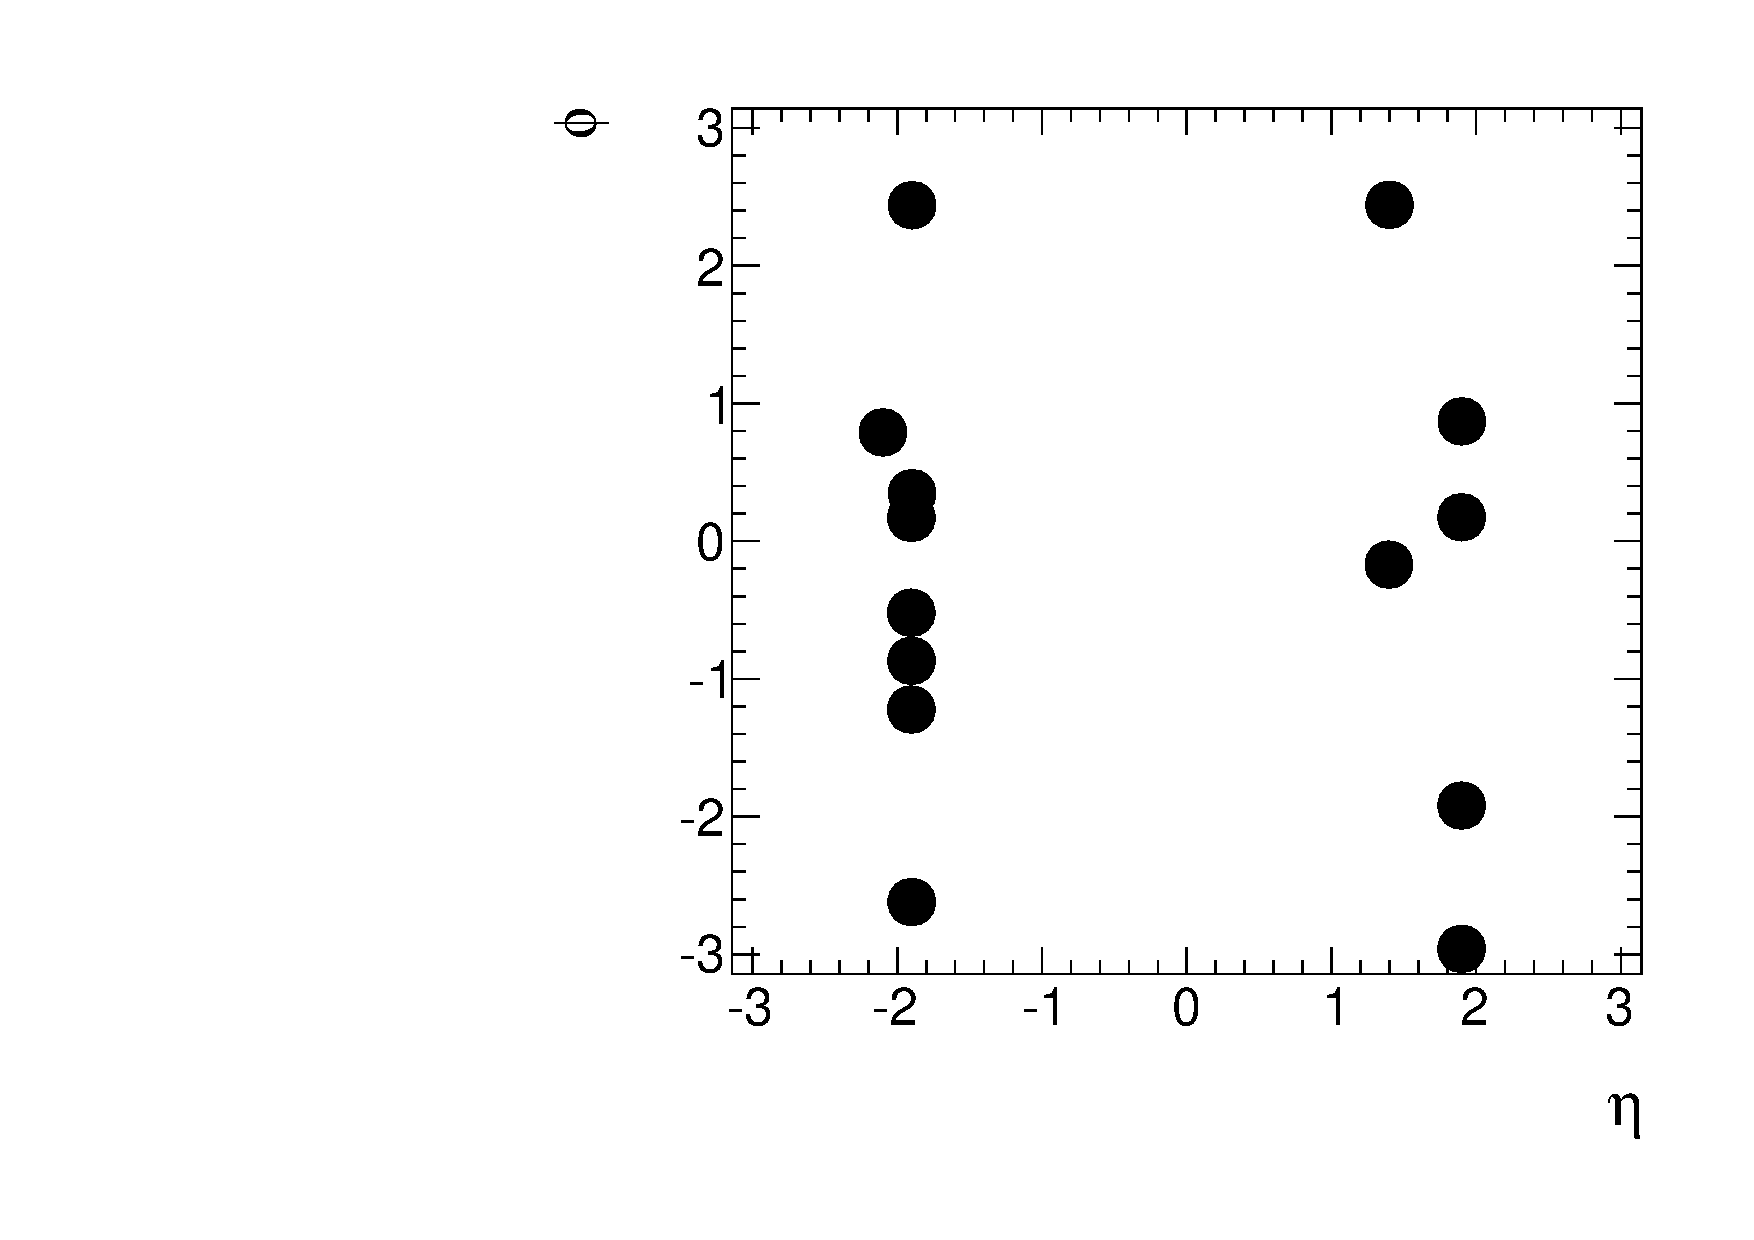
\includegraphics[width=0.49\textwidth]{figures/analysis/AnalysisSelection/BadCSCMap.pdf}
  \end{tabular}
  \caption{Visualisation of bad cathode strip chambers in the detector's $\phi - \eta$.}
  \label{fig:BadCSCMap}
\end{figure}

To summarise, the candidate track must fulfil the following selection criteria:
\begin{itemize}
\renewcommand{\labelitemi}{\footnotesize{\ding{118}}}
\item The track must not be within a cone of $\Delta R<0.15$ to a reconstructed standalone, tracker or global muon with a transverse momentum larger than 10\gev (see Section~\ref{FIXME} for details on the different muon definitions).
\item The track must not be within a cone of $\Delta R<0.15$ to a reconstructed electron with a transverse momentum larger than 10\gev (see Section~\ref{FIXME} for details on the electron reconstruction).
\item The track must not be within a cone of $\Delta R<0.15$ to a reconstructed tau with $\pt>20\gev$ and $|\eta|<2.3$ (see Section~\ref{FIXME} for details on the tau reconstruction). 
      Some loose isolation requirements are enforced to protect the tau reconstruction from jet contamination.
\item The track must not be within a cone of $\Delta R< 0.5$ to a reconstructed jet ($\pt>20\gev$ and $|\eta|<4.5$).
\item Veto tracks within a cone of $\Delta R<0.05$ to a dead or noisy ECAL cell (visualised in Fig.~\ref{fig:DeadECALmap}).
\item Veto tracks that point towards the direction of the ECAL intermodule gap listed in Table~\ref{tab:IntermoduleGaps}.
\item Veto tracks that point towards a bad CSC (visualised in Fig.~\ref{fig:BadCSCMap}).
\item Veto tracks that point towards the region between ECAL barrel and endcap at $1.42<|\eta|<1.65$
\end{itemize}
These lepton and jet veto selection requirements are of course highly suppressing the background emerging from real lepton/jet production like in \WJets events.
The discrimination power of the lepton and jet vetos is shown in Fig.~\ref{fig:TrackdRmin} where the minimum $\Delta R$ between the candidate track and a reconstructed electron, muon, tau or jet is shown.\\
\begin{figure}[!t]
  \centering 
  \begin{tabular}{c}
    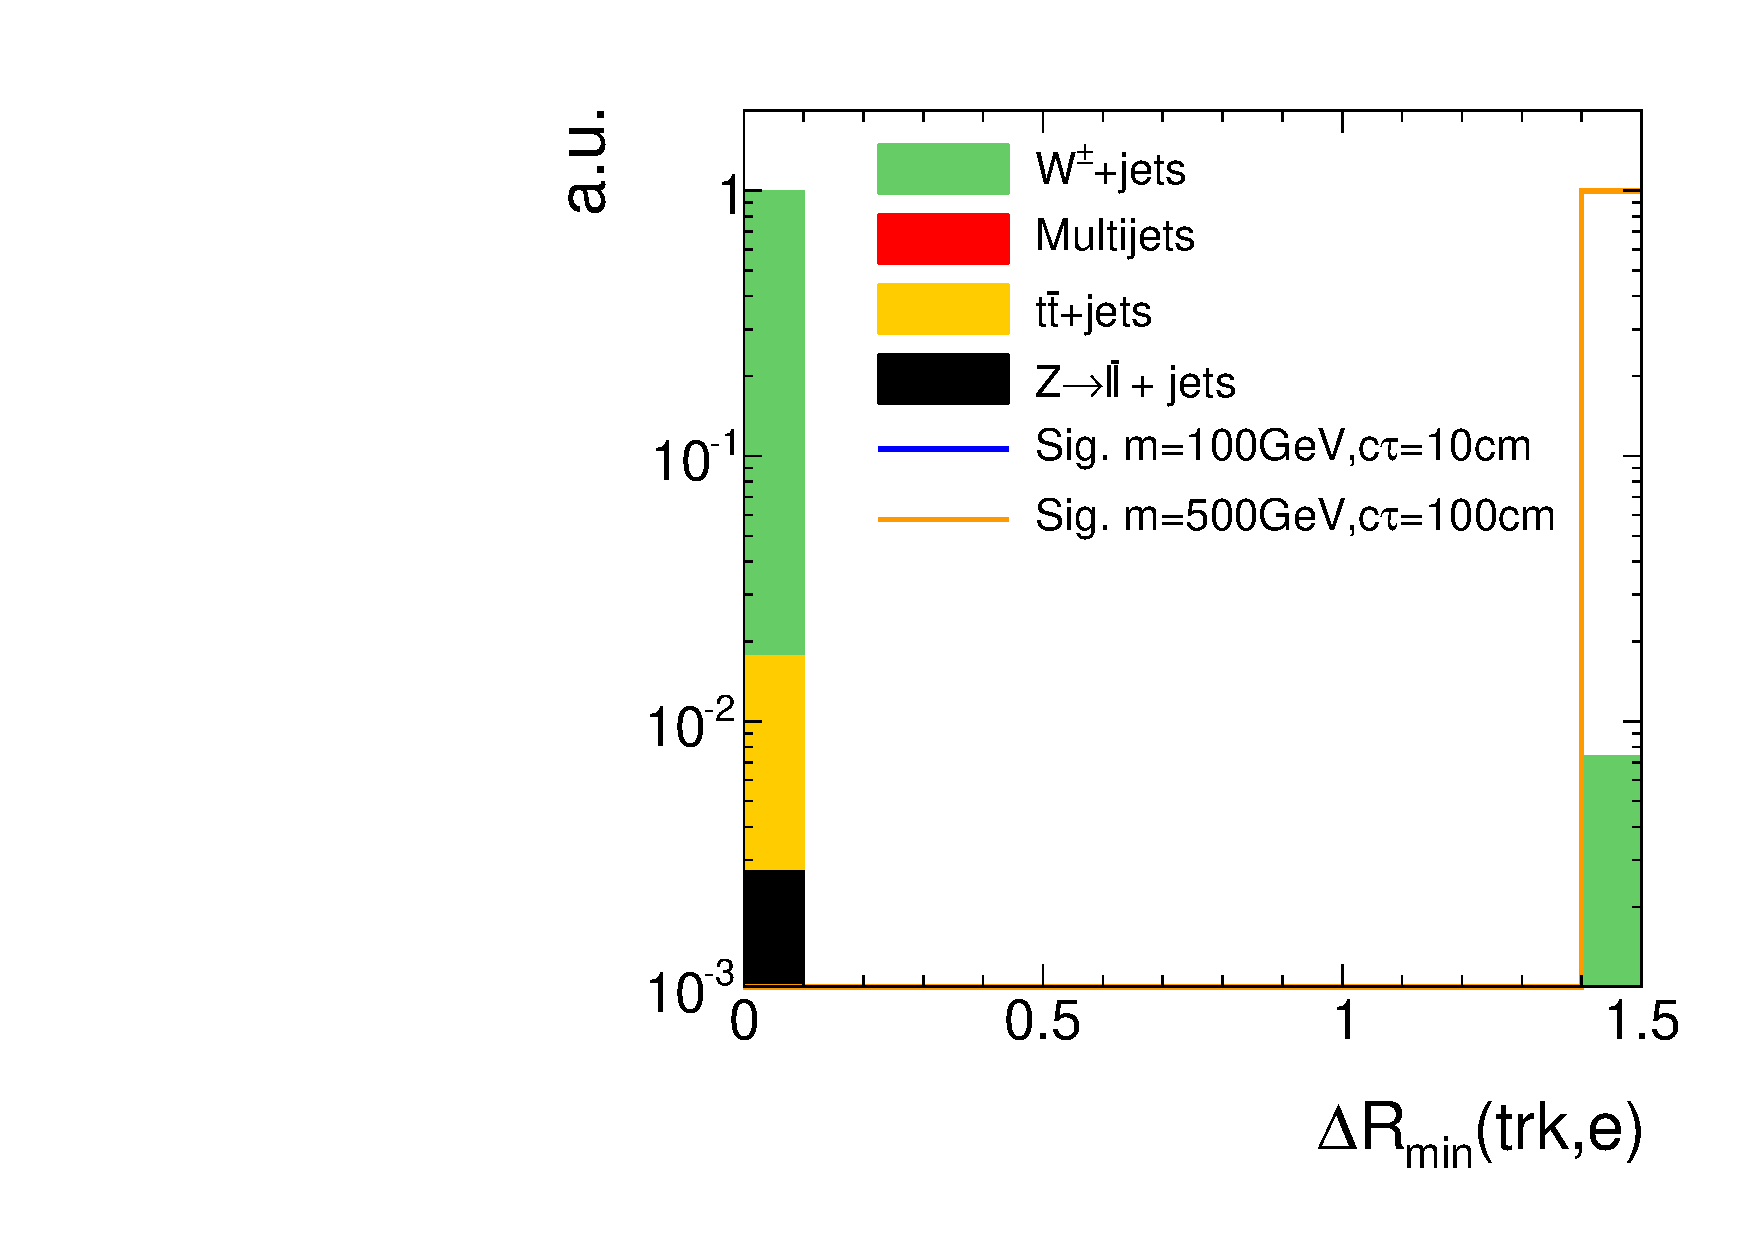
\includegraphics[width=0.49\textwidth]{figures/analysis/AnalysisSelection/htrackdRminElec_log.pdf}
    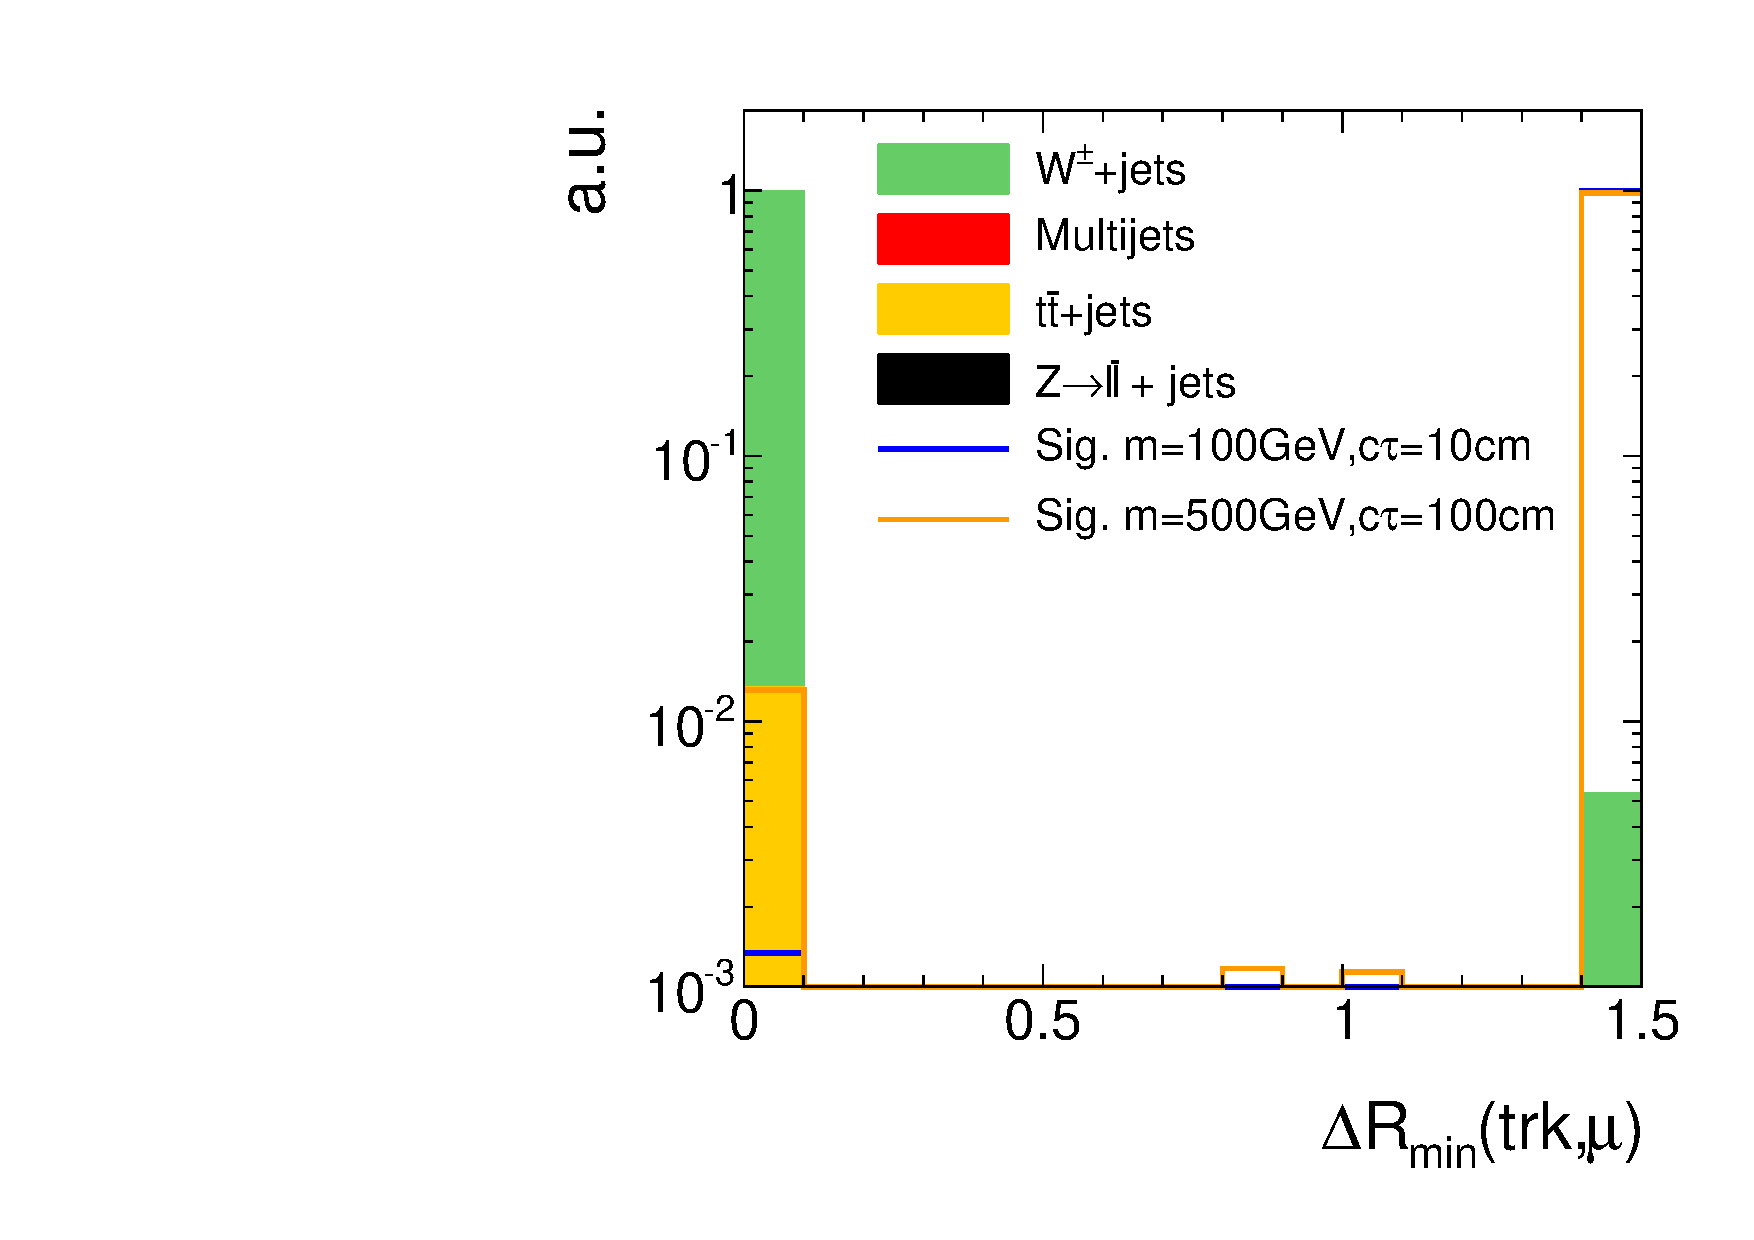
\includegraphics[width=0.49\textwidth]{figures/analysis/AnalysisSelection/htrackdRminMuon_log.pdf}\\

    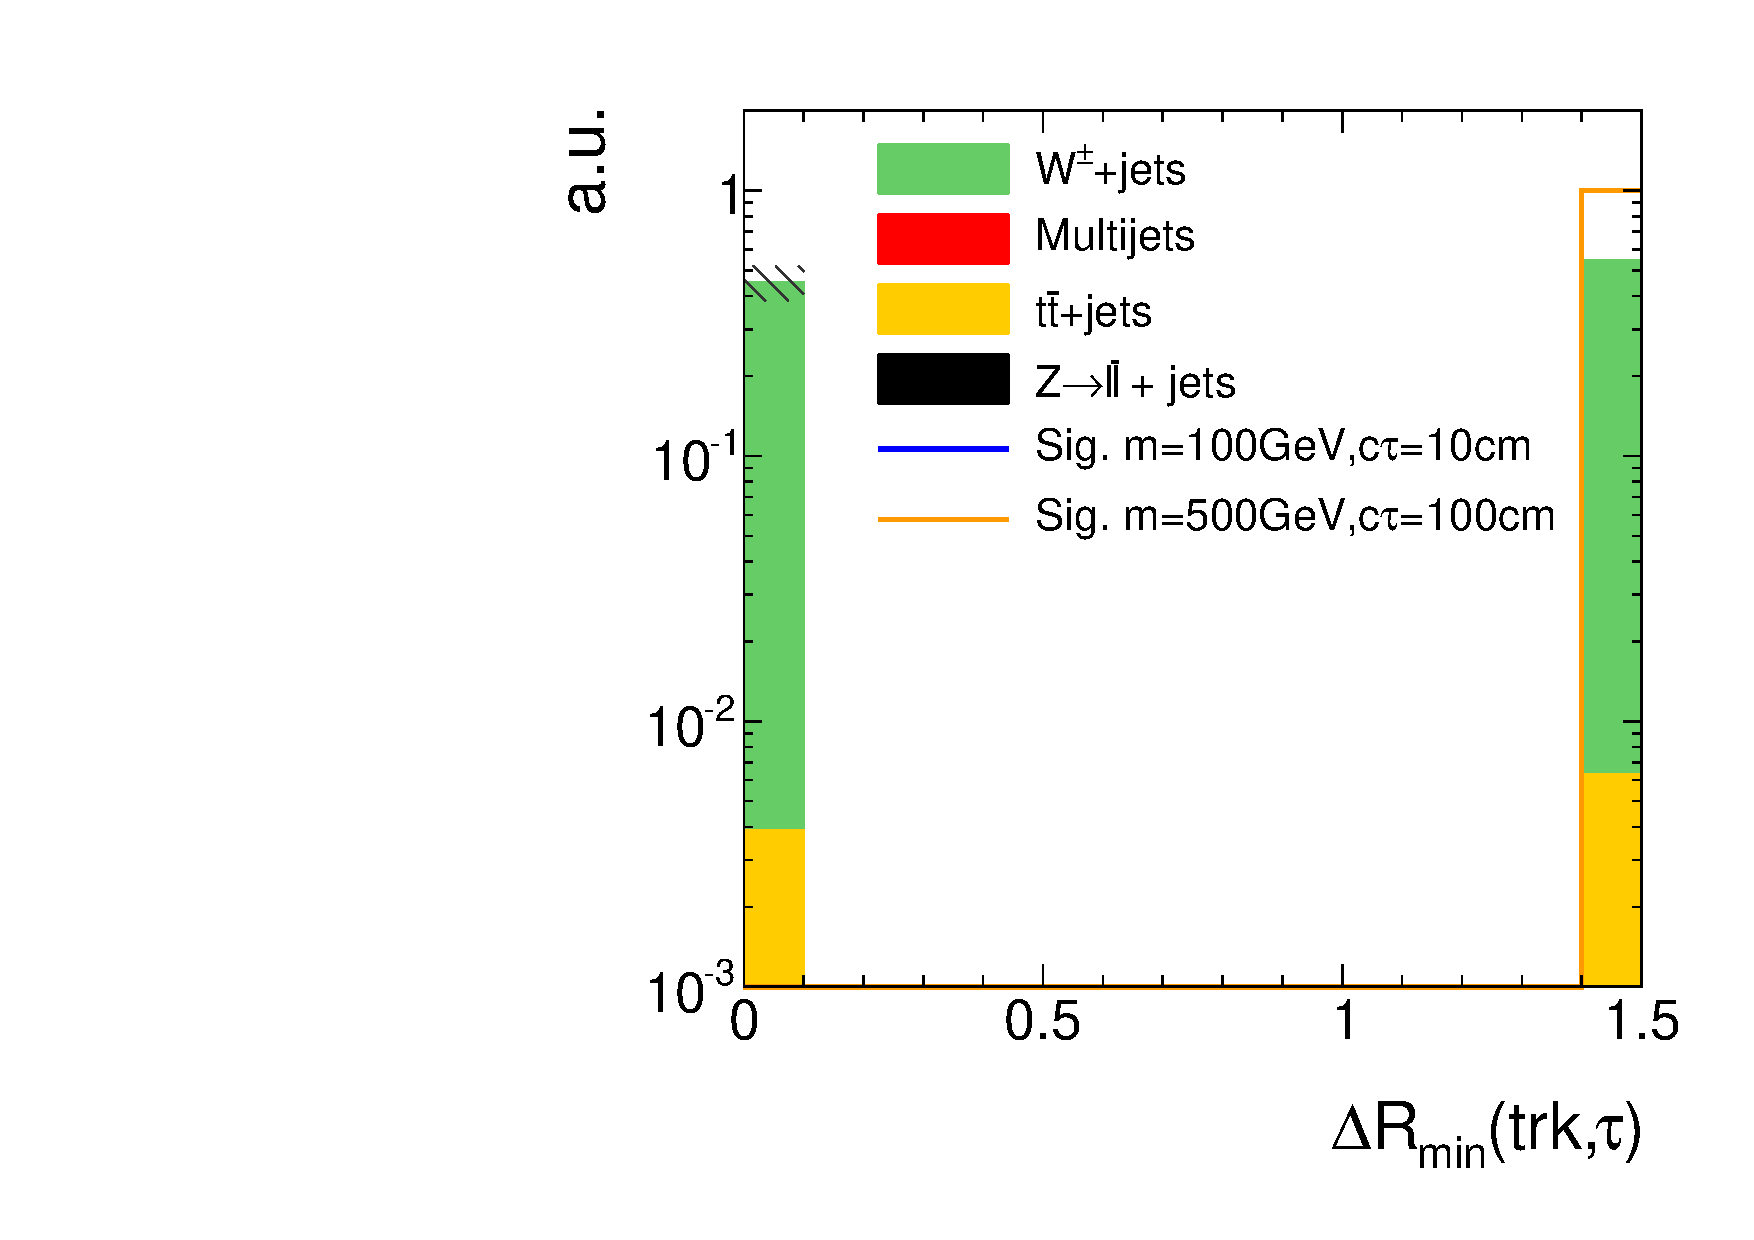
\includegraphics[width=0.49\textwidth]{figures/analysis/AnalysisSelection/htrackdRminTau_log.pdf}
    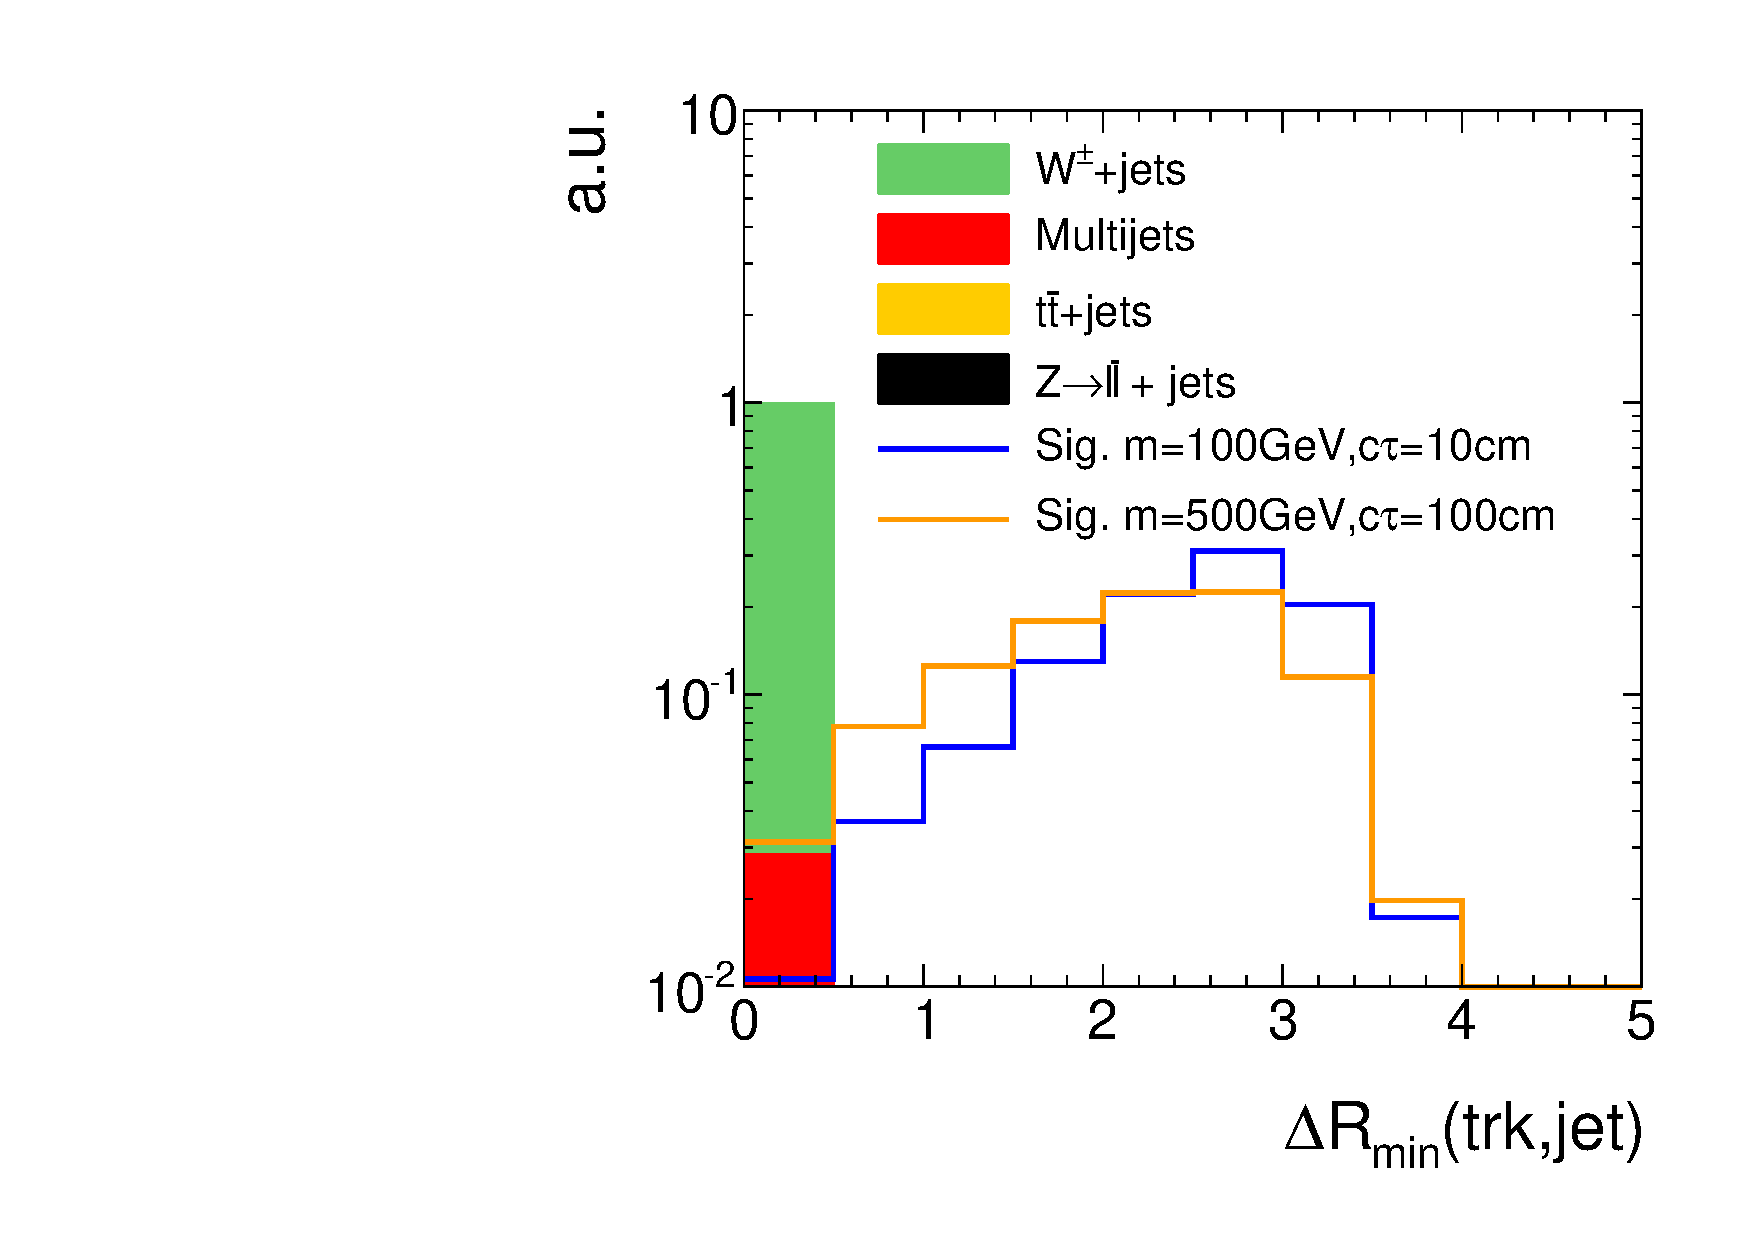
\includegraphics[width=0.49\textwidth]{figures/analysis/AnalysisSelection/htrackdRminJet_log.pdf}
  \end{tabular}
  \caption{The minimum $\Delta R$ between the candidate track and a reconstructed electron (top left), muon (top right), tau (bottom left) or jet (bottom right) 
           after the full candidate track selection cuts besides the one shown in the corresponding plot.}
  \label{fig:TrackdRmin}
\end{figure}


Finally, two further characteristics of chargino tracks are exploited.
As the chargino is produced in a very clean environment, the isolation of the track can discriminate signal against background events.

Furthermore, for charginos decaying inside the tracker there is no associated energy deposition in the calorimeters in the direction of the track.
This is a very pronounced characteristics of signal tracks.

The resulting selection cuts are as follows
\begin{itemize}
\renewcommand{\labelitemi}{\footnotesize{\ding{118}}}
\item No further substantial track activity (less than 10\%) is allowed in a cone of $\Delta R < 0.3$ around the candidate track: \mbox{$\sum \limits_{\Delta R < 0.3} \pt/p_{\text{T}}^{\text{cand}} < 0.1$}
\item Little calorimeter energy deposits (ECAL+HCAL) in a cone of $\Delta R < 0.5$ around the track: \mbox{$\ecalo<5\gev$}.
\end{itemize}
The discrimination power of these two variables is shown in Fig.~\ref{fig:TrackIso_Ecalo_After_Preselection}.\\
\begin{figure}[!t]
  \centering 
  \begin{tabular}{c}
    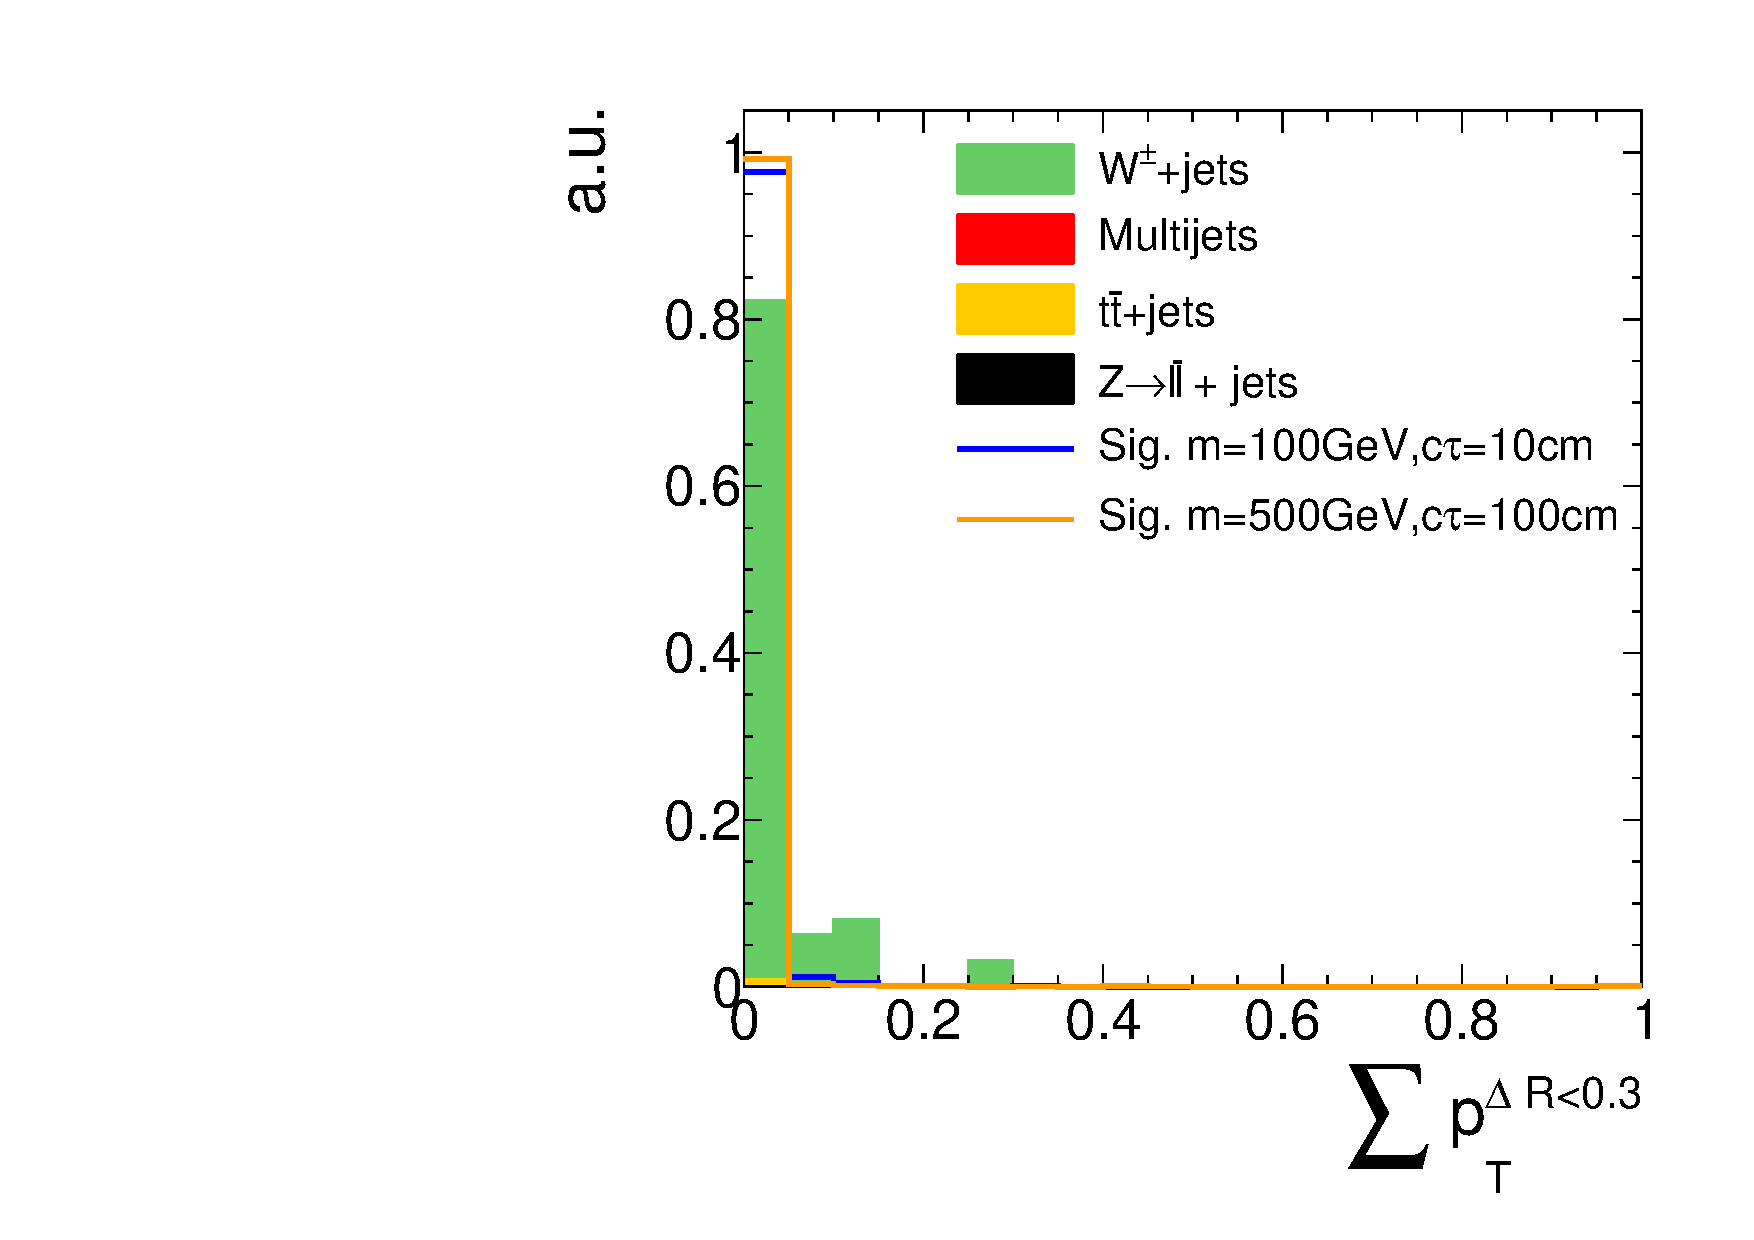
\includegraphics[width=0.49\textwidth]{figures/analysis/AnalysisSelection/chiTracksCandidateSelectionTrigger_2Signals_FullBkg/htrackIsolationSmallRange_lin.pdf}
    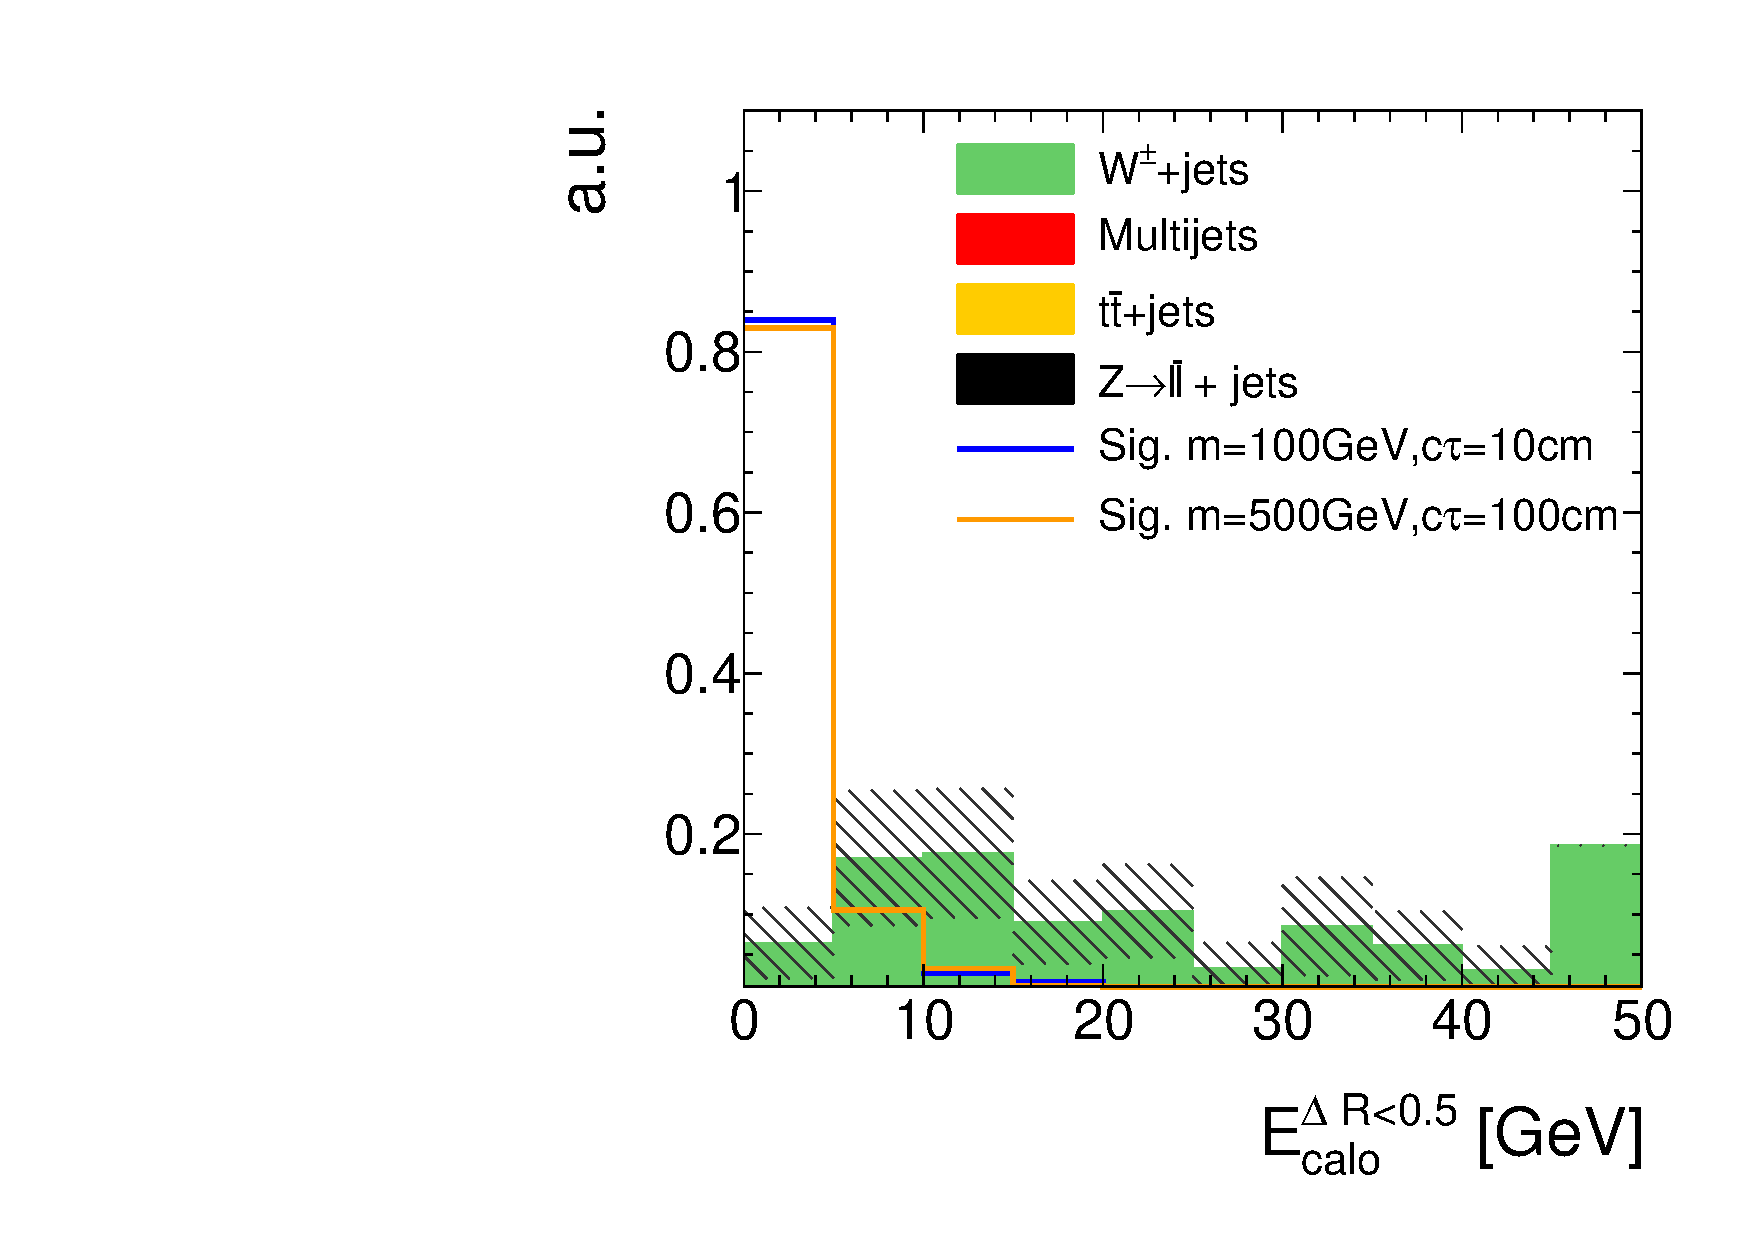
\includegraphics[width=0.49\textwidth]{figures/analysis/AnalysisSelection/chiTracksCandidateSelectionTrigger_2Signals_FullBkg/htrackCaloIsolation_lin.pdf}
  \end{tabular}
  \caption{Track isolation (left) and calorimeter energy deposits (right) of the candidate track after the full previous selection.}
  \label{fig:TrackIso_Ecalo_After_Preselection}
\end{figure}


As emphasised before, this analysis aims at being sensitive especially on shorter lifetimes.
Still, in order to allow for charginos decaying at any layer of the tracker, no explicit selection cut on the number of missing outer hits is required.
%For charginos with very short mean lifetimes it was checked, whether a sensitivity increase can be achieved by imposing a cut on $N_{\text{miss}}^{\text{outer}}$.
%However, this is not the case and therefore a selection in $N_{\text{miss}}^{\text{outer}}$ is not considered.


An overview over the full analysis preselection is given in Table~\ref{tab:SummaryCuts}. 
\renewcommand{\arraystretch}{1.39}
\begin{table}[!h]
\centering
\caption{Summary and categorisation of the analysis selection.}
\label{tab:SummaryCuts}
\makebox[0.99\textwidth]{
\begin{tabular}{l|l|l}
\multicolumn{3}{c}{} \\
\toprule
   
\multirow{3}{*}{Trigger}                                       &  \multicolumn{2}{l}{HLTMonoCentralPFJet80\_PFMETnoMu95\_NHEF0p95 }\\
                                                               &  \multicolumn{2}{l}{HLTMonoCentralPFJet80\_PFMETnoMu105\_NHEF0p95}\\
                                                               &  \multicolumn{2}{l}{HLT\_MET120\_HBHENoiseCleaned }\\\midrule

\multirow{4}{*}{\makecell[l]{Event-based \\ selection}}        &  \multirow{2}{*}{Trigger selection}   & \makecell[l]{$\ptfirstjet>100\gev$ \hfill with $|\eta_{\text{1.jet}}|<2.4$,  \\
                                                                                                                   \hfill $\text{CHF}_{\text{1.jet}}>0.2$, \\
                                                                                                                   \hfill $\text{CEF}_{\text{1.jet}}<0.5$, \\
                                                                                                                   \hfill $\text{NHF}_{\text{1.jet}}<0.7$, \\
                                                                                                                   \hfill $\text{NEF}_{\text{1.jet}}<0.7$\phantom{,}} \\
                                                               &                                       & $\met>100\gev$                                                  \\\cmidrule{2-3}
                                                               &  \multirow{2}{*}{QCD suppression}      & \makecell[l]{$\Delta\phi_{\text{max}} \left( \text{jet}_i, \text{jet}_j  \right)<2.7$  for all jets with \\ \hfill $\pt>20\gev$, $|\eta|<4.5$}\\
                                                               &                                       & \makecell[l]{$\Delta\phi_{\text{max}} \left( \text{jet}_i, \met  \right)>0.5$  for two leading jets}\\

\midrule

\multirow{18}{*}{\makecell[l]{Candidate track\\ selection}}   &  \multicolumn{2}{l}{$\geq1$ track that fulfils the following criteria:}\\\cmidrule{2-3}

                                                              &  \multirow{4}{*}{Good quality selection}   & high-purity as defined in~\cite{bib:CMS:Tracking_2010} \\
                                                              &                                            & $N_{\text{miss}}^{\text{middle/inner}}=0$\\
                                                              &                                            & $|d0|<0.02\cm$\\
                                                              &                                            & $|dz|<0.5\cm$\\\cmidrule{2-3}

                                                              &  \multirow{2}{*}{Kinematic selection}      & $|\eta|<2.1$ \\
                                                              &                                            & $\pt>10\gev$ \\\cmidrule{2-3}

                                                              &  \multirow{8}{*}{Lepton/jet veto}          & No muon within $\Delta R<0.15$ \\
                                                              &                                            & No electron within $\Delta R<0.15$ \\
                                                              &                                            & No tau within $\Delta R<0.15$ \\
                                                              &                                            & No jet within $\Delta R<0.5$ \\
                                                              &                                            & No dead/noisy ECAL cell within $\Delta R<0.05$  \\
                                                              &                                            & Not within an ECAL intermodule gap  \\
                                                              &                                            & Not within $1.42<|\eta|<1.65$ \\
                                                              &                                            & Not within $\Delta R<0.25$ to a bad CSC \\\cmidrule{2-3}

                                                              &  \multirow{2}{*}{Isolation selection}      & $\sum \limits_{\Delta R < 0.3} \pt/p_{\text{T}}^{\text{cand}} < 0.1$ \\
                                                              &                                            & $\ecalo<5\gev$ \\


\bottomrule
\end{tabular}}
\end{table}  
A summary table of the event yields after each selection step for the simulated background datasets and for some of the signal models can be found in Appendix~\ref{app:cutflow}.\\


Given the presented signal candidate selection, a set of two variables remain  that are highly discriminating:
The transverse momentum and the energy release per path length of the candidate track.
In Fig.~\ref{fig:PtAndIasAfterFullPreselection}, the distribution of the remaining two variables are shown after the application of the full signal candidate selection.
\begin{figure}[!h]
  \centering 
  \begin{tabular}{c}
    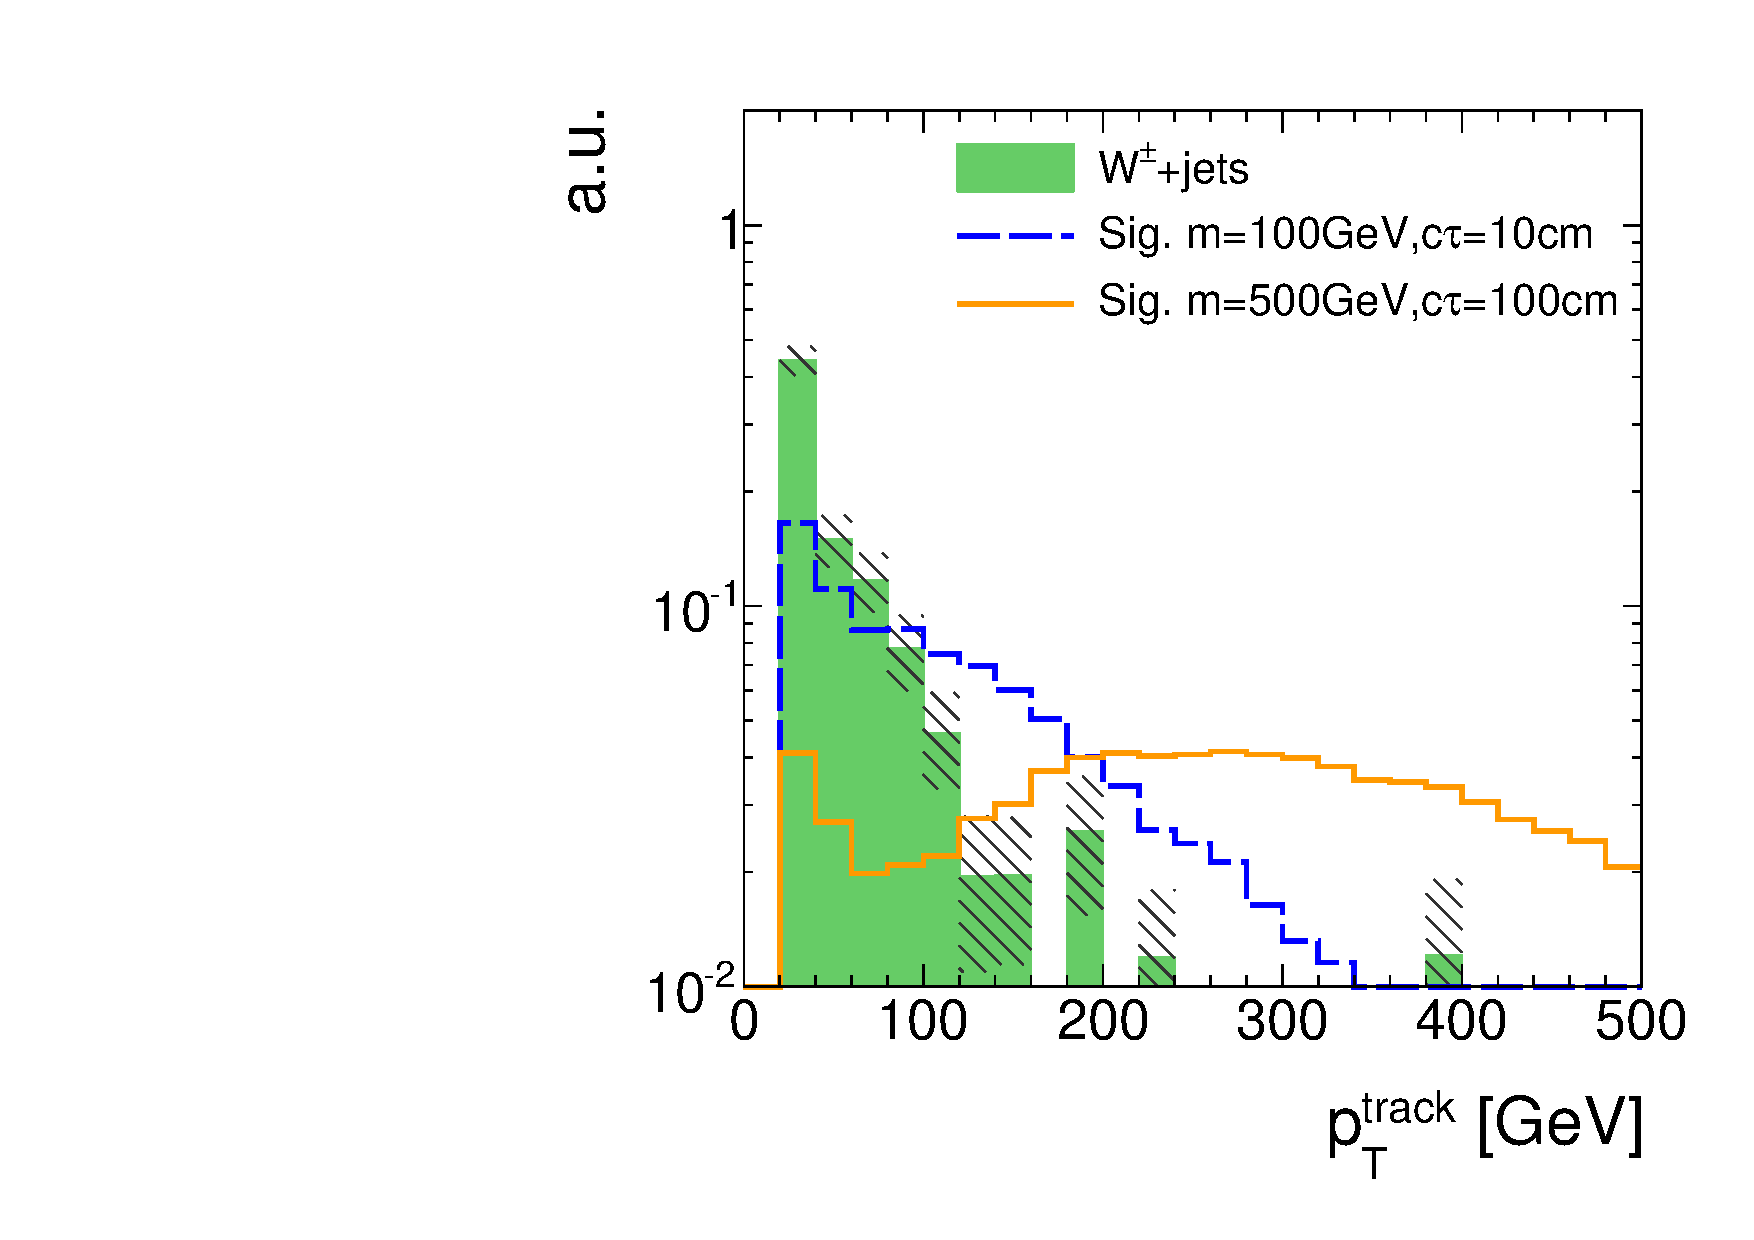
\includegraphics[width=0.49\textwidth]{figures/analysis/AnalysisSelection/chiTracksfullSelectionNoTriggerCuts_Wjets/htrackPtSmallRange_log.pdf}
    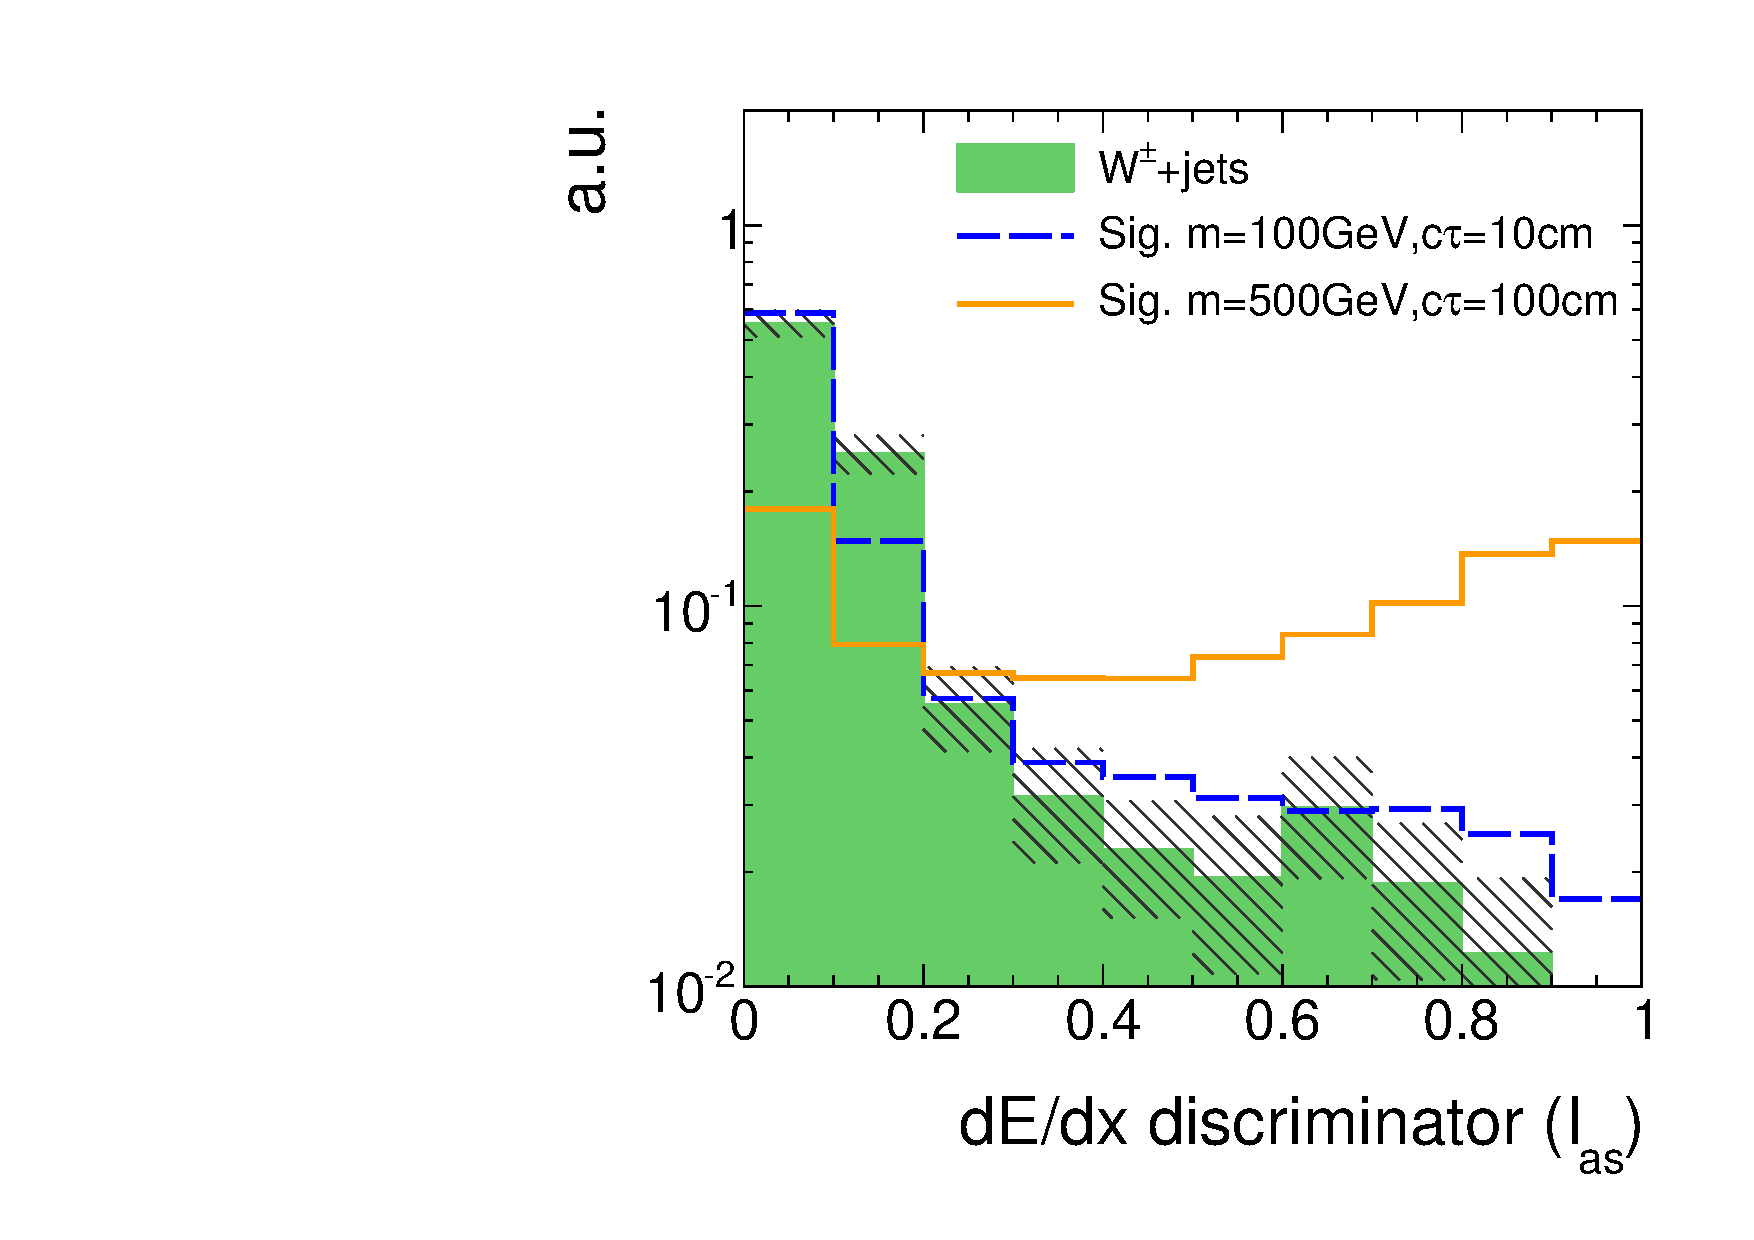
\includegraphics[width=0.49\textwidth]{figures/analysis/AnalysisSelection/chiTracksfullSelectionNoTriggerCuts_Wjets/htrackASmiSmallRange_log.pdf}
  \end{tabular}
  \caption{Candidate track \pt (left) and \ias (right) after the full signal candidate selection for signal and $\WJets$ events. 
           Because of the low statistical precision of the $\WJets$ sample, the trigger requirements are not applied.
           This does not influence the shape of the distributions since \met and \ptfirstjet are not expected to be correlated with the track characteristics.}
  \label{fig:PtAndIasAfterFullPreselection}
\end{figure}
These variables are used to optimise the sensitivity of the search.
The optimisation process will be explained in Section~\ref{sec:Optimisation}.
However, before the optimisation can be accomplished, a characterisation end estimation of the background is needed.
This topic will be discussed in the following section.

